\documentclass{article}\usepackage[]{graphicx}\usepackage[table]{xcolor}
% maxwidth is the original width if it is less than linewidth
% otherwise use linewidth (to make sure the graphics do not exceed the margin)
\makeatletter
\def\maxwidth{ %
  \ifdim\Gin@nat@width>\linewidth
    \linewidth
  \else
    \Gin@nat@width
  \fi
}
\makeatother

\definecolor{fgcolor}{rgb}{0.345, 0.345, 0.345}
\newcommand{\hlnum}[1]{\textcolor[rgb]{0.686,0.059,0.569}{#1}}%
\newcommand{\hlsng}[1]{\textcolor[rgb]{0.192,0.494,0.8}{#1}}%
\newcommand{\hlcom}[1]{\textcolor[rgb]{0.678,0.584,0.686}{\textit{#1}}}%
\newcommand{\hlopt}[1]{\textcolor[rgb]{0,0,0}{#1}}%
\newcommand{\hldef}[1]{\textcolor[rgb]{0.345,0.345,0.345}{#1}}%
\newcommand{\hlkwa}[1]{\textcolor[rgb]{0.161,0.373,0.58}{\textbf{#1}}}%
\newcommand{\hlkwb}[1]{\textcolor[rgb]{0.69,0.353,0.396}{#1}}%
\newcommand{\hlkwc}[1]{\textcolor[rgb]{0.333,0.667,0.333}{#1}}%
\newcommand{\hlkwd}[1]{\textcolor[rgb]{0.737,0.353,0.396}{\textbf{#1}}}%
\let\hlipl\hlkwb

\usepackage{framed}
\makeatletter
\newenvironment{kframe}{%
 \def\at@end@of@kframe{}%
 \ifinner\ifhmode%
  \def\at@end@of@kframe{\end{minipage}}%
  \begin{minipage}{\columnwidth}%
 \fi\fi%
 \def\FrameCommand##1{\hskip\@totalleftmargin \hskip-\fboxsep
 \colorbox{shadecolor}{##1}\hskip-\fboxsep
     % There is no \\@totalrightmargin, so:
     \hskip-\linewidth \hskip-\@totalleftmargin \hskip\columnwidth}%
 \MakeFramed {\advance\hsize-\width
   \@totalleftmargin\z@ \linewidth\hsize
   \@setminipage}}%
 {\par\unskip\endMakeFramed%
 \at@end@of@kframe}
\makeatother

\definecolor{shadecolor}{rgb}{.97, .97, .97}
\definecolor{messagecolor}{rgb}{0, 0, 0}
\definecolor{warningcolor}{rgb}{1, 0, 1}
\definecolor{errorcolor}{rgb}{1, 0, 0}
\newenvironment{knitrout}{}{} % an empty environment to be redefined in TeX

\usepackage{alltt}

\usepackage[utf8]{inputenc}
\usepackage{float}
\usepackage{graphicx}
\usepackage{booktabs}
\usepackage[table]{xcolor}
\usepackage{comment}
\usepackage{caption}

\newenvironment{tablas}[2]
{\begin{table}[H]
		\centering
		\caption{#1}
		#2
		\caption*{Fuente trabajo de campo}}
	{\end{table}}


\newenvironment{fotos}[2]
{\begin{figure}[H]
	\centering
	\caption{#1}
	\includegraphics[width=7cm, height=7cm]{H:/Gore Cusco/Geragri/programa/analisis datos/fotos/#2.jpg}
	\caption*{Fuente: trabajo de campo}}
{\end{figure}}


\newenvironment{graficas}[2]
{\begin{figure}[H]
		\centering
		\caption{#1}
		#2
		\caption*{Fuente trabajo de campo}}
{\end{figure}}
\IfFileExists{upquote.sty}{\usepackage{upquote}}{}
\begin{document}



modificacion desde github desktop\\
Se realizara el analisis de las encuestas de todas la encuestas realizadas en el trabajo de campo.\\
\begin{table}[H]
  \centering
  \caption{Edad de los encuestados}

\begin{tabular}{lcl}
\toprule
\cellcolor[HTML]{87A96B}{\textcolor{black}{\textbf{Rango}}} & \cellcolor[HTML]{87A96B}{\textcolor{black}{\textbf{Conteo}}} & \cellcolor[HTML]{87A96B}{\textcolor{black}{\textbf{Porcentaje}}}\\
\midrule
(23.9,33.3] & 28 & 6.35\\
(33.3,42.6] & 54 & 12.24\\
(42.6,51.9] & 87 & 19.73\\
(51.9,61.1] & 127 & 28.80\\
(61.1,70.4] & 97 & 22.00\\
\addlinespace
(70.4,79.7] & 35 & 7.94\\
(79.7,89.1] & 13 & 2.95\\
\bottomrule
\end{tabular}

  \caption*{Fuente trabajo de campo}
\end{table}
Aca ira la interpretacion de la tabla
\begin{figure}[H]
  \centering
  \caption{Porcentaje de edad de los encuestados}
\begin{knitrout}
\definecolor{shadecolor}{rgb}{0.969, 0.969, 0.969}\color{fgcolor}
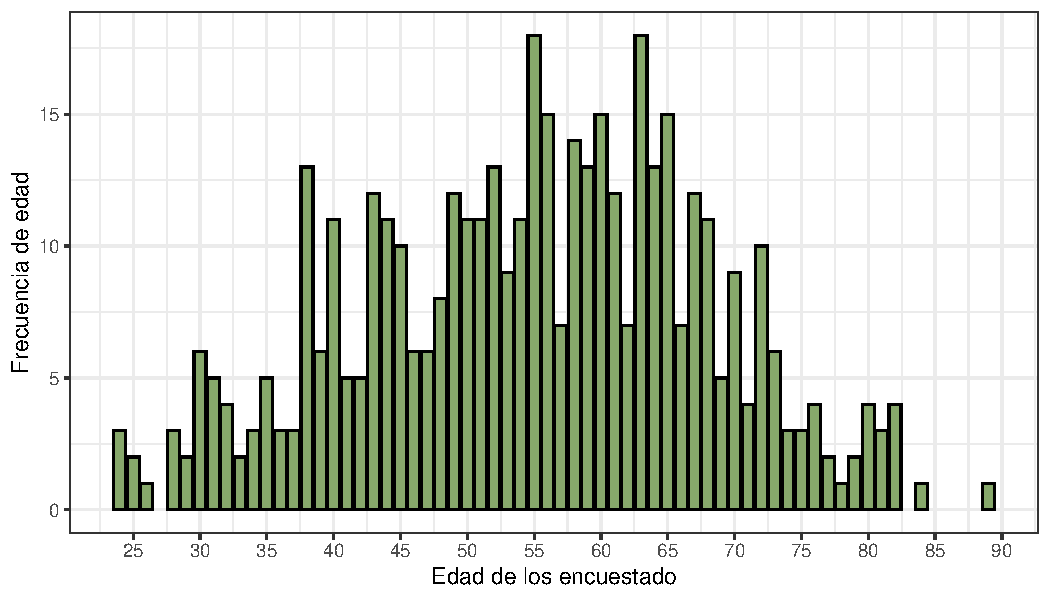
\includegraphics[width=\maxwidth]{figure/fig_uno-1} 
\end{knitrout}
  \caption*{Fuente: trabajo de campo}
\end{figure}

\begin{fotos}
{Aplicacion de encuestas}{1}
\end{fotos}


Se analizara el genero de los encuestados
\begin{table}[H]
  \centering
  \caption{Genero de los encuestados}

\begin{tabular}{lcl}
\toprule
\cellcolor[HTML]{87A96B}{\textcolor{black}{\textbf{GENERO}}} & \cellcolor[HTML]{87A96B}{\textcolor{black}{\textbf{Conteo}}} & \cellcolor[HTML]{87A96B}{\textcolor{black}{\textbf{Porcentaje}}}\\
\midrule
MUJER & 213 & 47.97\\
VARON & 231 & 52.03\\
\bottomrule
\end{tabular}

  \caption*{Fuente: Trabajo de campo}
\end{table}  

\begin{figure}[H]
  \centering
  \caption{Frecuencia del genero de los encuestados}
\begin{knitrout}
\definecolor{shadecolor}{rgb}{0.969, 0.969, 0.969}\color{fgcolor}
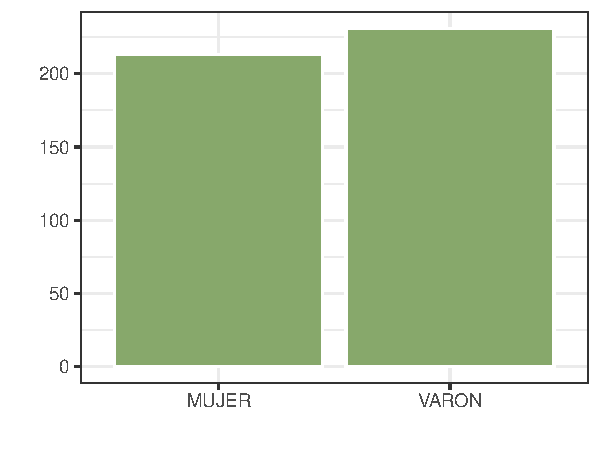
\includegraphics[width=\maxwidth]{figure/fig_dos-1} 
\end{knitrout}
  \caption*{Fuente: Trabajo de campo}
\end{figure}

\begin{table}[H]
  \centering
  \caption{Grado de instruccion}

\begin{tabular}{lcl}
\toprule
\cellcolor[HTML]{87A96B}{\textcolor{black}{\textbf{Grado}}} & \cellcolor[HTML]{87A96B}{\textcolor{black}{\textbf{Conteo}}} & \cellcolor[HTML]{87A96B}{\textcolor{black}{\textbf{Porcentaje}}}\\
\midrule
NINGUNO & 95 & 22.73\\
PRIMARIA & 209 & 50.00\\
SECUNDARIA & 106 & 25.36\\
SUPERIOR & 5 & 1.20\\
TECNICO & 3 & 0.72\\
\bottomrule
\end{tabular}


  \caption*{Fuente: Trabajo de campo}
\end{table}
\begin{figure}[H]
  \centering
  \caption{Distribucion del grado de instruccion}
\begin{knitrout}
\definecolor{shadecolor}{rgb}{0.969, 0.969, 0.969}\color{fgcolor}
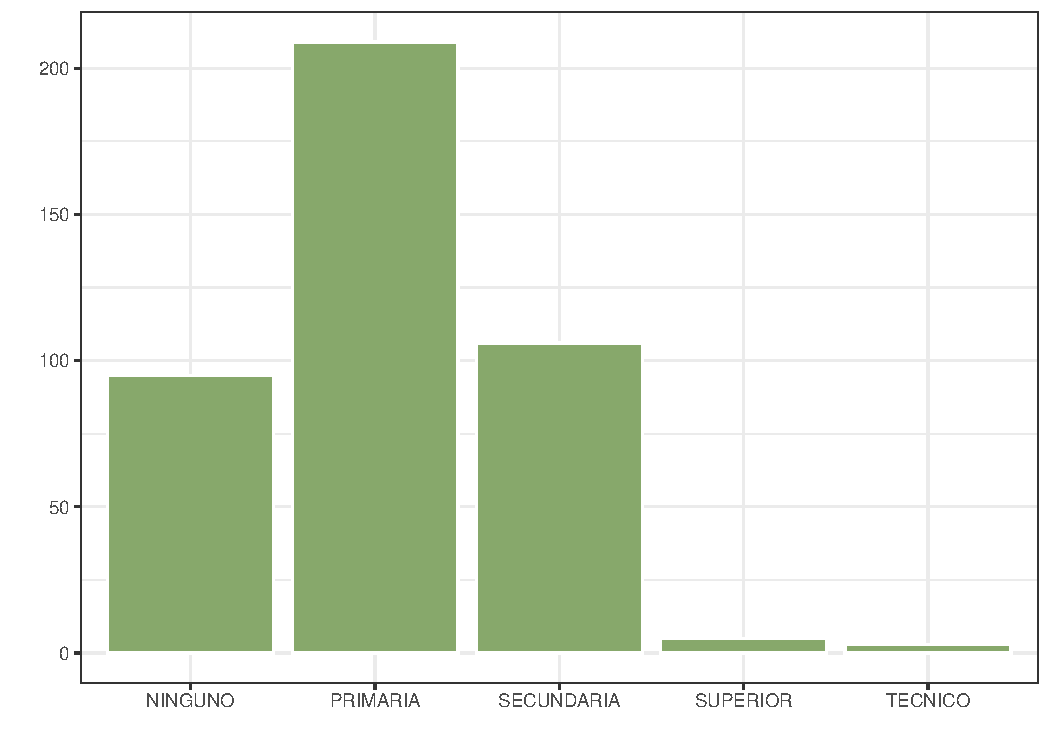
\includegraphics[width=\maxwidth]{figure/fig_tres-1} 
\end{knitrout}
  \caption*{Fuente: Trabajo de campo}
\end{figure}

\begin{fotos}
{Aplicacion de encuestas}{2}
\end{fotos}


\begin{table}[H]
  \centering
  \caption{Tipo de ingreso familiar}

\begin{tabular}{lcl}
\toprule
\cellcolor[HTML]{87A96B}{\textcolor{black}{\textbf{Ingreso}}} & \cellcolor[HTML]{87A96B}{\textcolor{black}{\textbf{Conteo}}} & \cellcolor[HTML]{87A96B}{\textcolor{black}{\textbf{Porcentaje}}}\\
\midrule
ANUAL & 240 & 61.22\\
MENSUAL & 126 & 32.14\\
QUINCENAL & 20 & 5.10\\
SEMANAL & 6 & 1.53\\
\bottomrule
\end{tabular}

  \caption*{Fuente: Trabajo de campo}
\end{table}


\begin{figure}[H]
  \centering
  \caption{Distribucion del tipo de ingreso familiar}
\begin{knitrout}
\definecolor{shadecolor}{rgb}{0.969, 0.969, 0.969}\color{fgcolor}
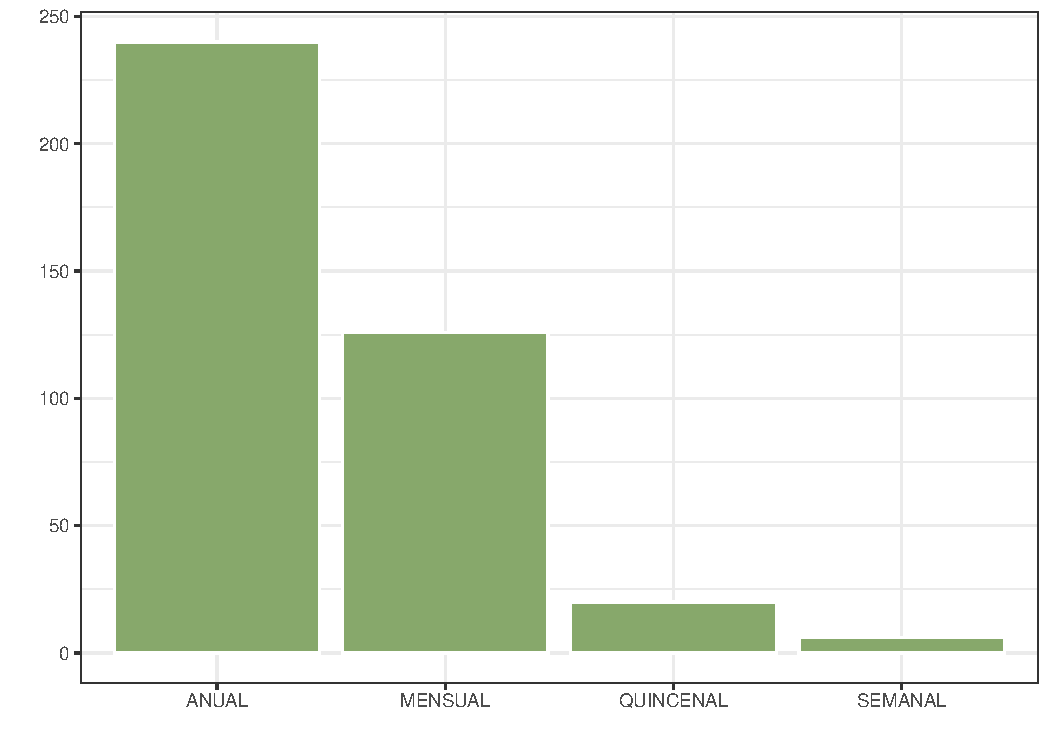
\includegraphics[width=\maxwidth]{figure/fig_cinco-1} 
\end{knitrout}
  \caption*{Fuente: Trabajo de campo}
\end{figure}
\begin{fotos}
{Aplicacion de encuestas}{3}
\end{fotos}


\begin{table}[H]
  \centering
  \caption{Ingreso familiar}

\begin{tabular}{lcl}
\toprule
\cellcolor[HTML]{87A96B}{\textcolor{black}{\textbf{Ingreso\_familiar}}} & \cellcolor[HTML]{87A96B}{\textcolor{black}{\textbf{Conteo}}} & \cellcolor[HTML]{87A96B}{\textcolor{black}{\textbf{Porcentaje}}}\\
\midrule
Mayor a S/1500 & 29 & 7.51\\
S/100 a S/500 & 269 & 69.69\\
S/501 a S/950 & 51 & 13.21\\
S/951 a S/1500 & 37 & 9.59\\
\bottomrule
\end{tabular}

  \caption*{Fuente: Trabajo de campo}
\end{table}


\begin{figure}[H]
  \centering
  \caption{Distribucion del tipo de ingreso familiar}
\begin{knitrout}
\definecolor{shadecolor}{rgb}{0.969, 0.969, 0.969}\color{fgcolor}
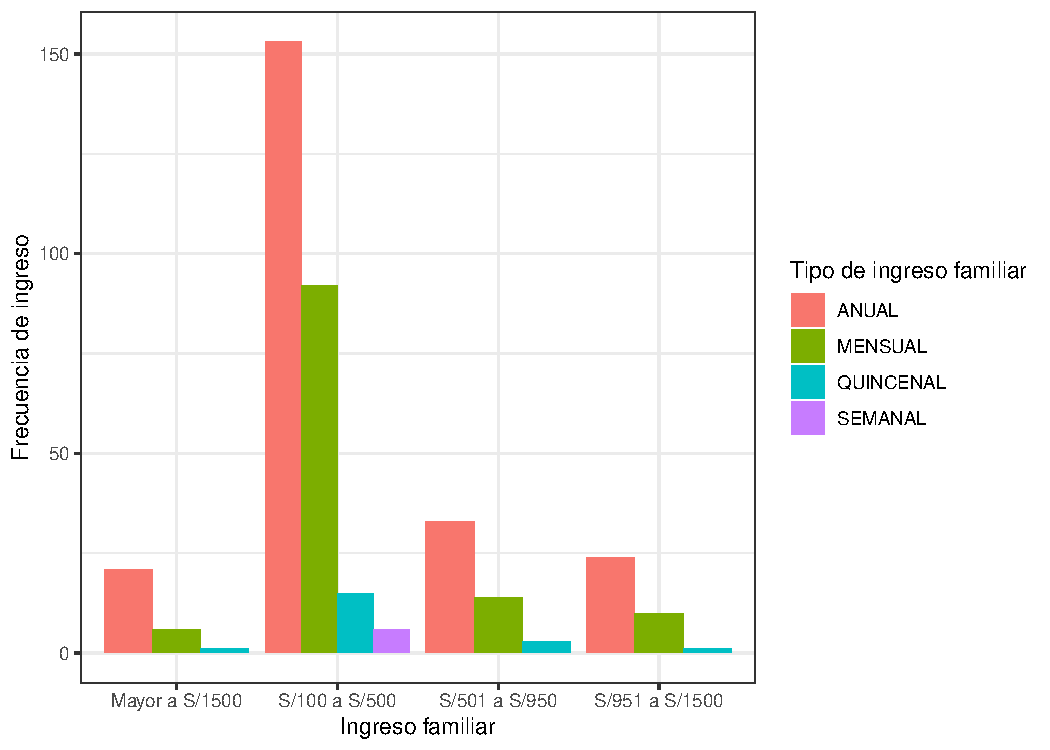
\includegraphics[width=\maxwidth]{figure/fig_seis-1} 
\end{knitrout}
  \caption*{Fuente: Trabajo de campo}
\end{figure}

\begin{fotos}
{Sensibililzacion a los beneficiarios}{4}
\end{fotos}


\begin{table}[H]
  \centering
  \caption{Numero de integrantes que conforman su familia}

\begin{tabular}{lcl}
\toprule
\cellcolor[HTML]{87A96B}{\textcolor{black}{\textbf{Integrantes}}} & \cellcolor[HTML]{87A96B}{\textcolor{black}{\textbf{Conteo}}} & \cellcolor[HTML]{87A96B}{\textcolor{black}{\textbf{Porcentaje}}}\\
\midrule
3 A 5 PERSONAS & 228 & 51.35\\
MAS DE 6 PERSONAS & 41 & 9.23\\
MENOS DE 2 PERSONAS & 175 & 39.41\\
\bottomrule
\end{tabular}


  \caption*{Fuente: Trabajo de campo}
\end{table}

\begin{figure}[H]
  \centering
  \caption{Numero de integrantes que conforman su familia}
\begin{knitrout}
\definecolor{shadecolor}{rgb}{0.969, 0.969, 0.969}\color{fgcolor}
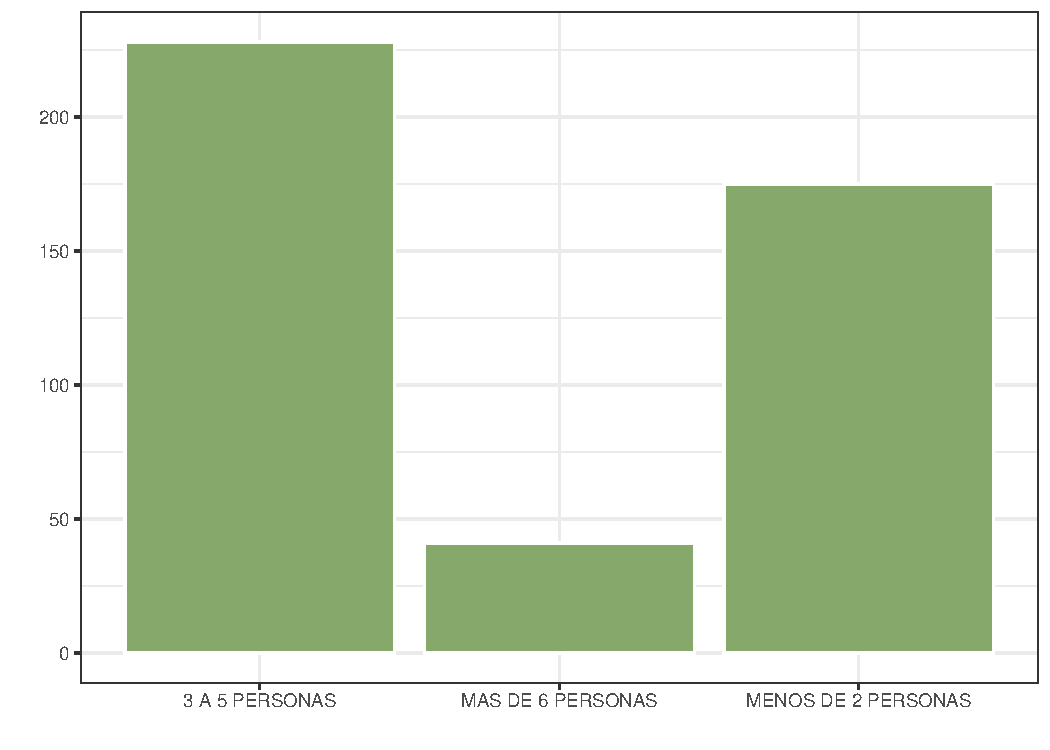
\includegraphics[width=\maxwidth]{figure/fig_siete-1} 
\end{knitrout}
  \caption*{Fuente: Trabajo de campo}
\end{figure}
\begin{fotos}
{Aplicacion de encuestas en el area de influencia}{5}
\end{fotos}


\begin{table}[H]
  \centering
  \caption{Actividad economica a la que se dedica}

\begin{tabular}{lcl}
\toprule
\cellcolor[HTML]{87A96B}{\textcolor{black}{\textbf{Actividad}}} & \cellcolor[HTML]{87A96B}{\textcolor{black}{\textbf{Conteo}}} & \cellcolor[HTML]{87A96B}{\textcolor{black}{\textbf{Porcentaje}}}\\
\midrule
AGRICULTOR & 146 & 32.74\\
AGROPECUARIO & 156 & 34.98\\
AMA DE CASA & 126 & 28.25\\
COMERCIANTE & 6 & 1.35\\
PECUARIO & 8 & 1.79\\
\addlinespace
TRABAJADOR PUBLICO & 4 & 0.90\\
\bottomrule
\end{tabular}

  \caption*{Fuente: Trabajo de campo}
\end{table}

\begin{figure}[H]
  \centering
  \caption{Actividad economica a la que se dedica}
\begin{knitrout}
\definecolor{shadecolor}{rgb}{0.969, 0.969, 0.969}\color{fgcolor}
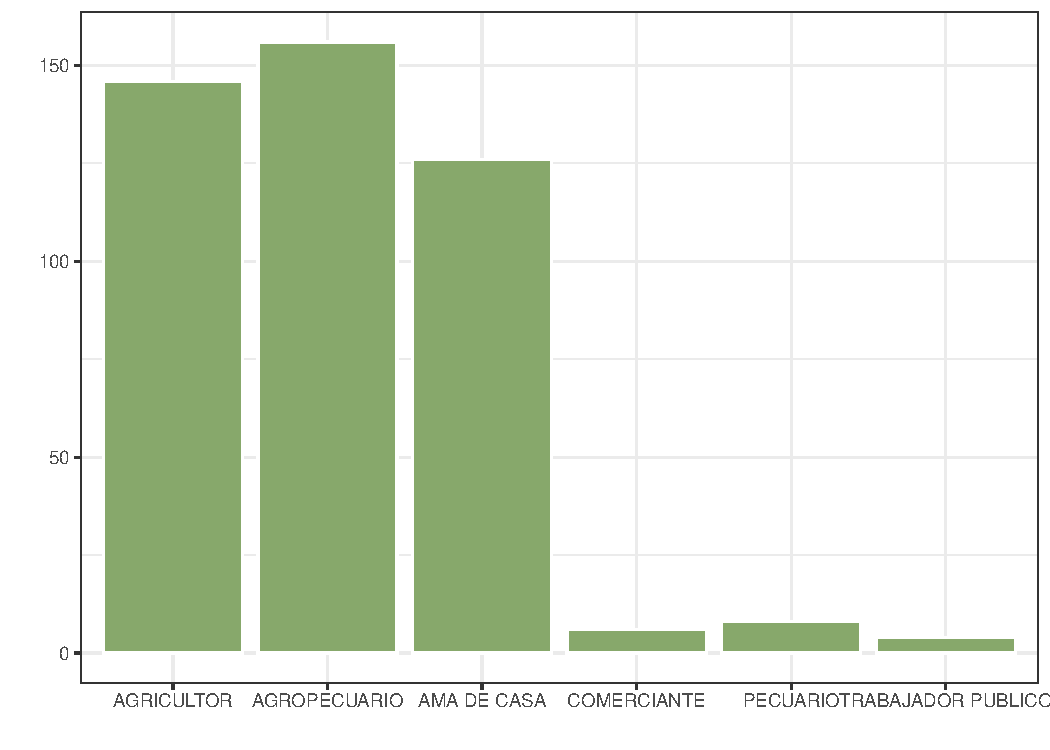
\includegraphics[width=\maxwidth]{figure/fig_ocho-1} 
\end{knitrout}
  \caption*{Fuente: Trabajo de campo}
\end{figure}
\begin{fotos}
{Aplicacion de encuestas en el area de influencia}{6}
\end{fotos}


\begin{table}[H]
  \centering
  \caption{Cuenta con el servicio de agua potable}

\begin{tabular}{lcl}
\toprule
\cellcolor[HTML]{87A96B}{\textcolor{black}{\textbf{Agua}}} & \cellcolor[HTML]{87A96B}{\textcolor{black}{\textbf{Conteo}}} & \cellcolor[HTML]{87A96B}{\textcolor{black}{\textbf{Porcentaje}}}\\
\midrule
NO & 3 & 0.67\\
SI & 445 & 99.33\\
\bottomrule
\end{tabular}

  \caption*{Fuente: Trabajo de campo}
\end{table}

\begin{figure}[H]
  \centering
  \caption{Cuenta con el servicio de agua potable}
\begin{knitrout}
\definecolor{shadecolor}{rgb}{0.969, 0.969, 0.969}\color{fgcolor}
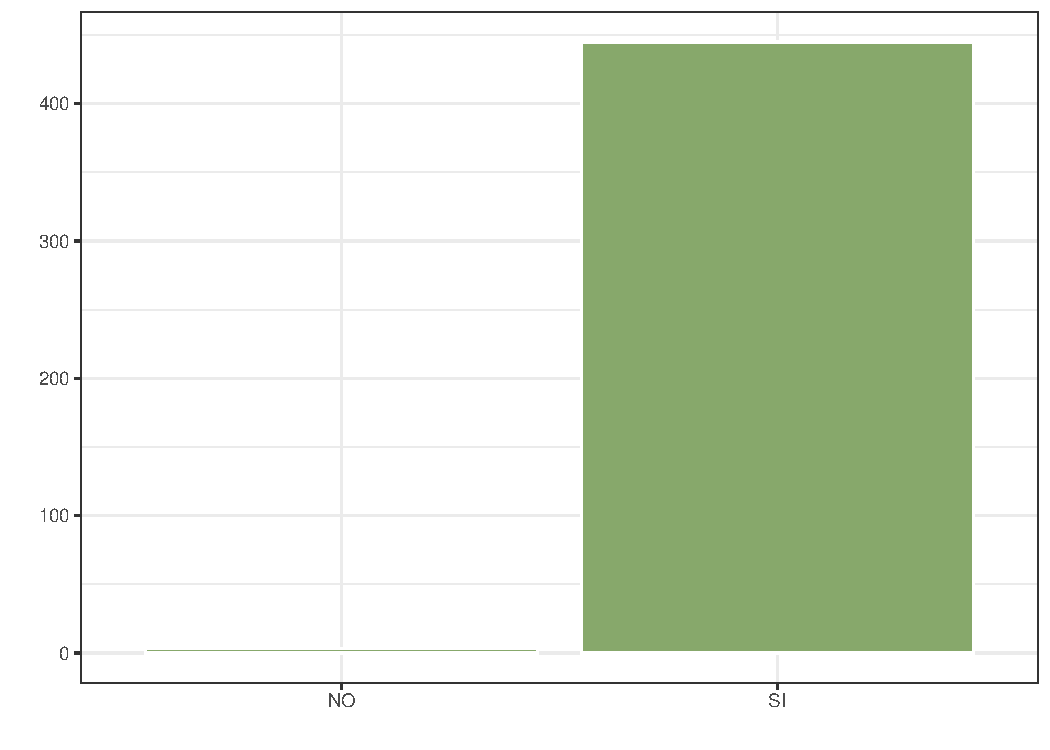
\includegraphics[width=\maxwidth]{figure/fig_nueve-1} 
\end{knitrout}
  \caption*{Fuente: Trabajo de campo}
\end{figure}

\begin{fotos}
{Aplicacion de encuestas en el area de influencia}{7}
\end{fotos}


\begin{table}[H]
  \centering
  \caption{Tipo de agua que consume}

\begin{tabular}{lcl}
\toprule
\cellcolor[HTML]{87A96B}{\textcolor{black}{\textbf{Agua\_que\_consume}}} & \cellcolor[HTML]{87A96B}{\textcolor{black}{\textbf{Conteo}}} & \cellcolor[HTML]{87A96B}{\textcolor{black}{\textbf{Porcentaje}}}\\
\midrule
CLORADA & 327 & 75.00\\
POTABLE & 91 & 20.87\\
SIN TRATAR & 18 & 4.13\\
\bottomrule
\end{tabular}

  \caption*{Fuente: Trabajo de campo}
\end{table}

\begin{figure}[H]
  \centering
  \caption{Tipo de agua que consume}
\begin{knitrout}
\definecolor{shadecolor}{rgb}{0.969, 0.969, 0.969}\color{fgcolor}
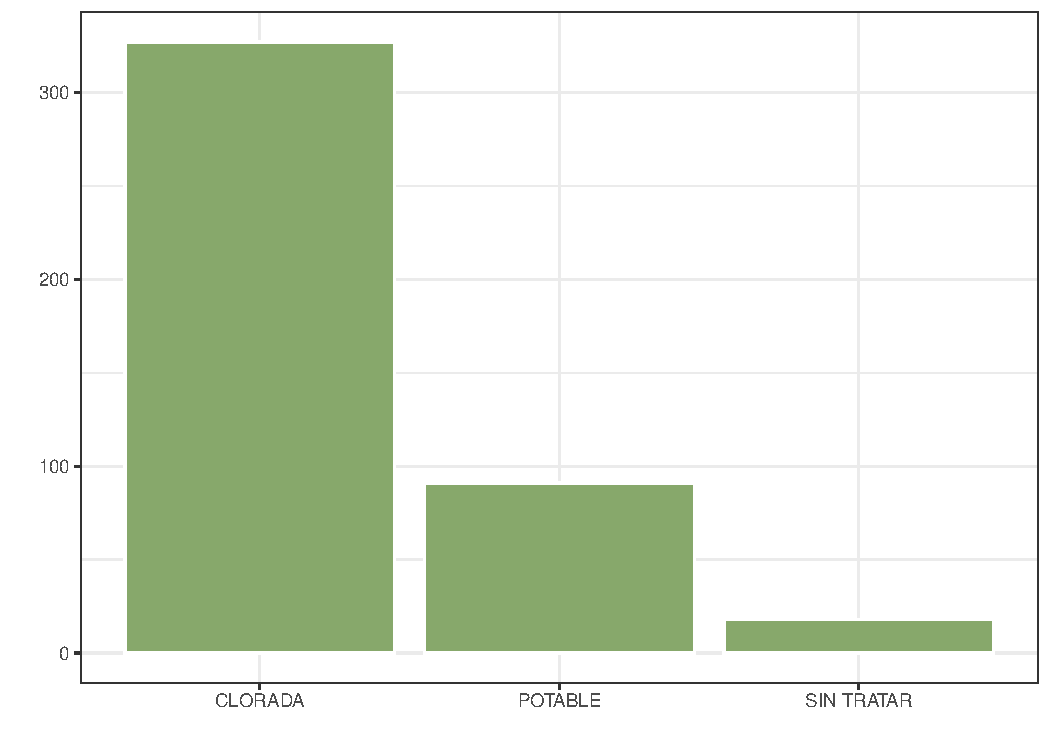
\includegraphics[width=\maxwidth]{figure/fig_diez-1} 
\end{knitrout}
  \caption*{Fuente: Trabajo de campo}
\end{figure}

\begin{fotos}
{sensibilizacion a la poblacion}{8}
\end{fotos}




\begin{table}[H]
  \centering
  \caption{Fuente de agua}

\begin{tabular}{lcl}
\toprule
\cellcolor[HTML]{87A96B}{\textcolor{black}{\textbf{Abastecimiento\_agua}}} & \cellcolor[HTML]{87A96B}{\textcolor{black}{\textbf{Conteo}}} & \cellcolor[HTML]{87A96B}{\textcolor{black}{\textbf{Porcentaje}}}\\
\midrule
MANTIAL & 323 & 72.91\\
PILON DE USO PUBLICO & 13 & 2.93\\
RED PUBLICA & 94 & 21.22\\
RIO O RIACHUELO & 13 & 2.93\\
\bottomrule
\end{tabular}

  \caption*{Fuente: Trabajo de campo}
\end{table}

\begin{figure}[H]
  \centering
  \caption{Fuente de agua}
\begin{knitrout}
\definecolor{shadecolor}{rgb}{0.969, 0.969, 0.969}\color{fgcolor}
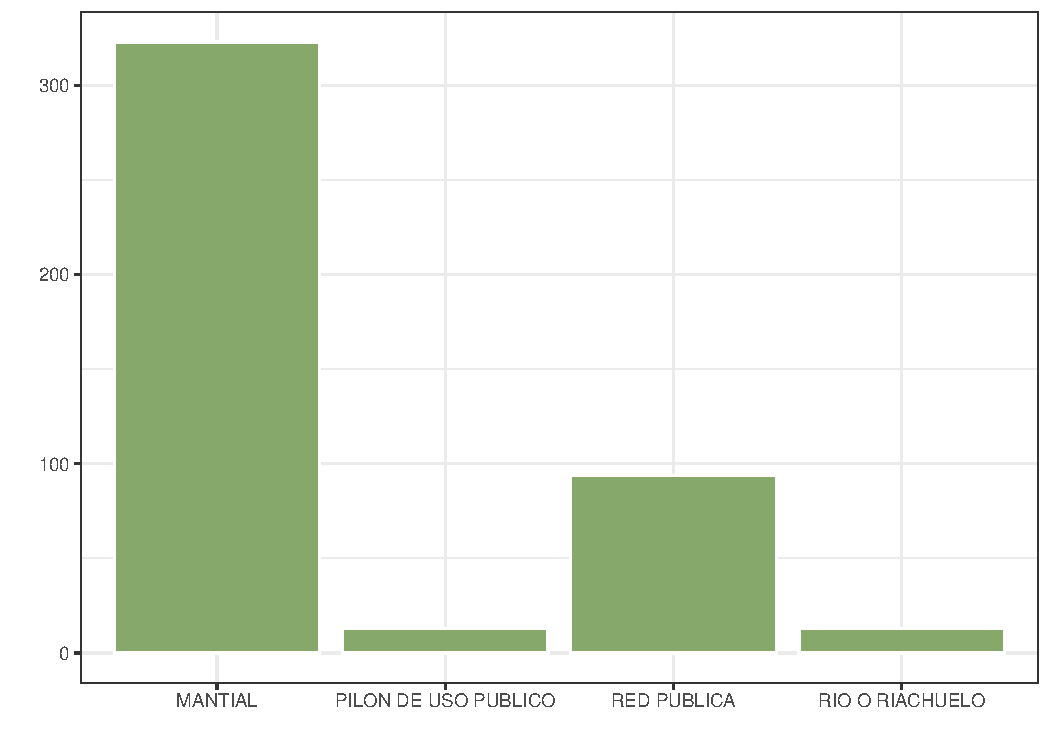
\includegraphics[width=\maxwidth]{figure/fig_once-1} 
\end{knitrout}
  \caption*{Fuente: Trabajo de campo}
\end{figure}
\begin{fotos}
{sensibilizacion a la poblacion}{9}
\end{fotos}

\begin{table}[H]
  \centering
  \caption{Energia electrica}

\begin{tabular}{lcl}
\toprule
\cellcolor[HTML]{87A96B}{\textcolor{black}{\textbf{Electricidad}}} & \cellcolor[HTML]{87A96B}{\textcolor{black}{\textbf{Conteo}}} & \cellcolor[HTML]{87A96B}{\textcolor{black}{\textbf{Porcentaje}}}\\
\midrule
NO & 26 & 5.83\\
SI & 420 & 94.17\\
\bottomrule
\end{tabular}

  \caption*{Fuente: Trabajo de campo}
\end{table}

\begin{figure}[H]
  \centering
  \caption{Energia electrica}
\begin{knitrout}
\definecolor{shadecolor}{rgb}{0.969, 0.969, 0.969}\color{fgcolor}
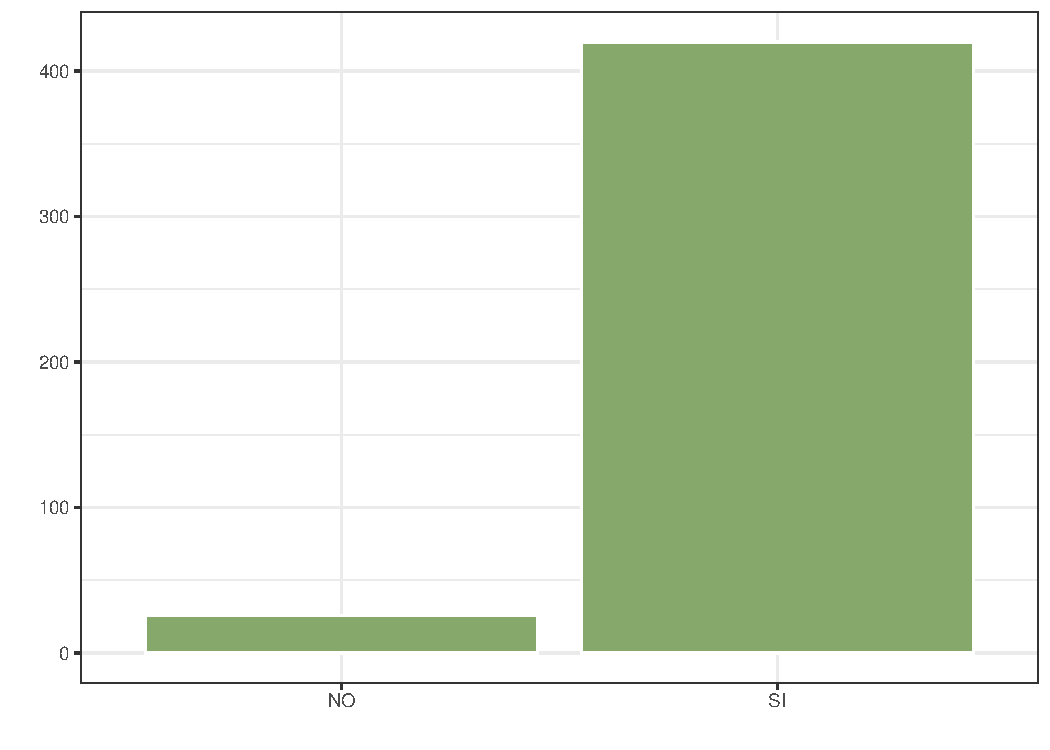
\includegraphics[width=\maxwidth]{figure/fig_doce-1} 
\end{knitrout}
  \caption*{Fuente: Trabajo de campo}
\end{figure}

\begin{fotos}
{sensibilizacion a la poblacion}{10}
\end{fotos}

\begin{comment}
\begin{table}[H]
  \centering
  \caption{Energia electrica}

  \caption*{Fuente: Trabajo de campo}
\end{table}

\begin{figure}[H]
  \centering
  \caption{Energia electrica}

  \caption*{Fuente: Trabajo de campo}
\end{figure}


%\begin{fotos}
%{sensibilizacion a la poblacion}{11}
%\end{fotos}
\end{comment}

\begin{table}[H]
  \centering
  \caption{Persona que trabaja en la parcela}

\begin{tabular}{lcl}
\toprule
\cellcolor[HTML]{87A96B}{\textcolor{black}{\textbf{Trabaja}}} & \cellcolor[HTML]{87A96B}{\textcolor{black}{\textbf{Conteo}}} & \cellcolor[HTML]{87A96B}{\textcolor{black}{\textbf{Porcentaje}}}\\
\midrule
OTRO & 4 & 0.89\\
UN AMIGO & 5 & 1.12\\
UN FAMILIAR & 35 & 7.83\\
USTED MISMO & 403 & 90.16\\
\bottomrule
\end{tabular}

  \caption*{Fuente: Trabajo de campo}
\end{table}

\begin{figure}[H]
  \centering
  \caption{Persona que trabaja en la parcela}
\begin{knitrout}
\definecolor{shadecolor}{rgb}{0.969, 0.969, 0.969}\color{fgcolor}
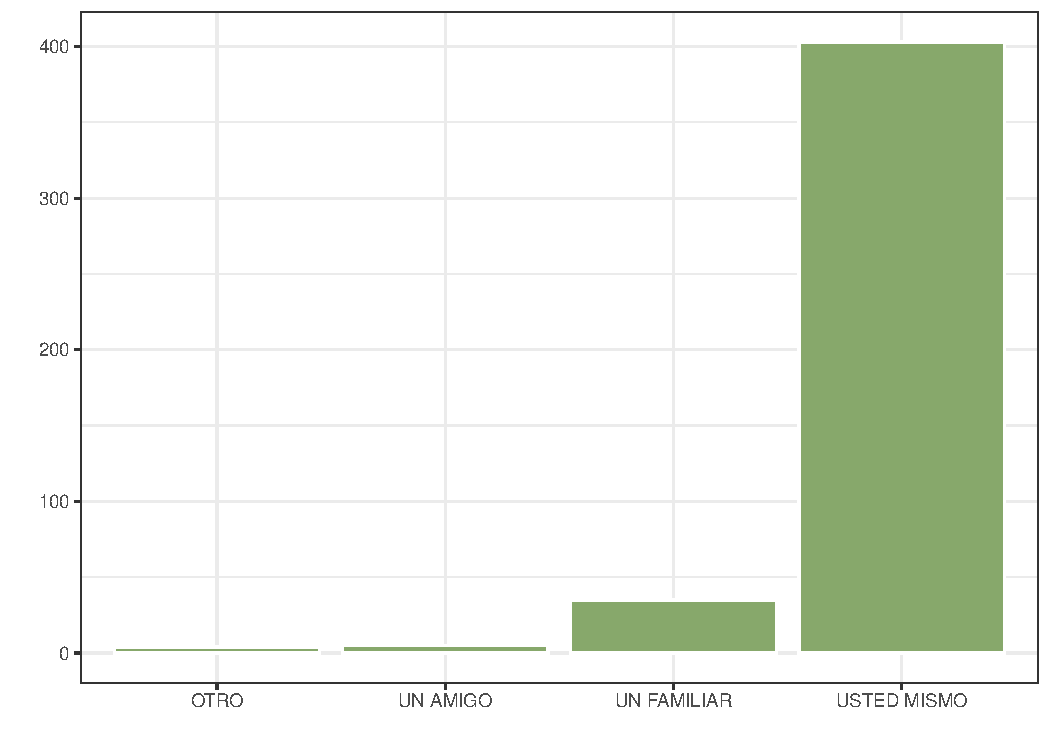
\includegraphics[width=\maxwidth]{figure/fig_catorce-1} 
\end{knitrout}
  \caption*{Fuente: Trabajo de campo}
\end{figure}

\begin{fotos}
{sensibilizacion a la poblacion}{12}
\end{fotos}


\begin{tablas}
{uso de la parcela en el ultimo año}{

\begin{tabular}{lcl}
\toprule
\cellcolor[HTML]{87A96B}{\textcolor{black}{\textbf{Uso\_parcela}}} & \cellcolor[HTML]{87A96B}{\textcolor{black}{\textbf{Conteo}}} & \cellcolor[HTML]{87A96B}{\textcolor{black}{\textbf{Porcentaje}}}\\
\midrule
CULTIVOS PERMANENTES & 252 & 57.27\\
CULTIVOS TRANSITORIOS & 165 & 37.50\\
PASTOS NATURALES & 23 & 5.23\\
\bottomrule
\end{tabular}

}
\end{tablas}

\begin{graficas}
{uso de la parcela en el ultimo año}{
\begin{knitrout}
\definecolor{shadecolor}{rgb}{0.969, 0.969, 0.969}\color{fgcolor}
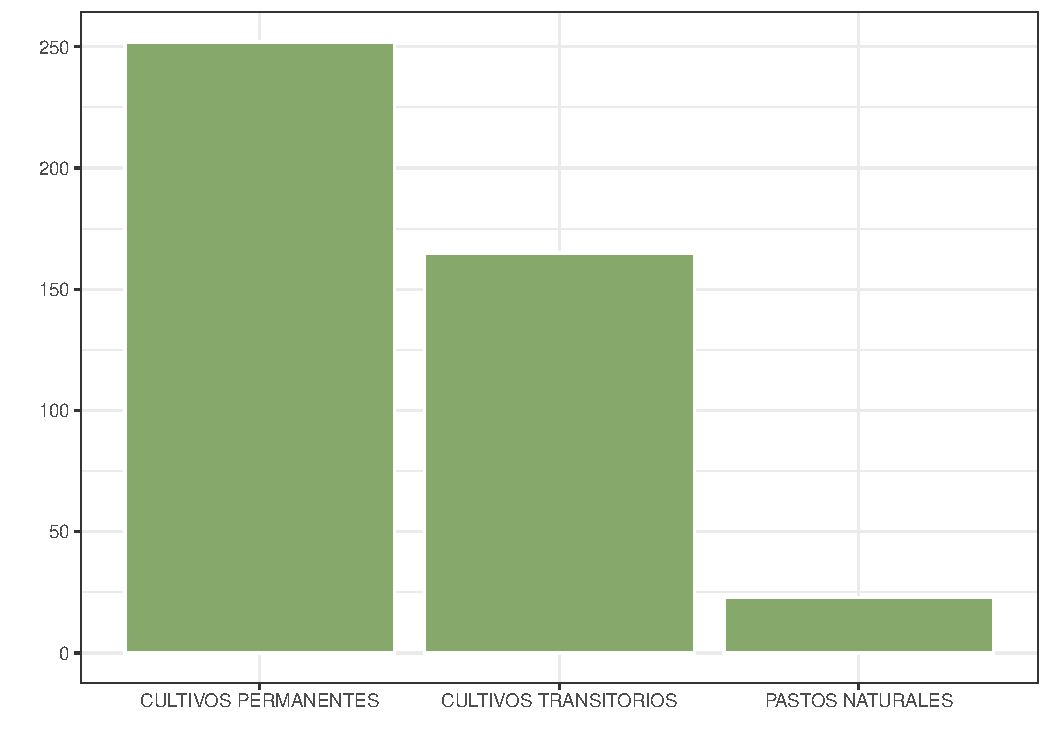
\includegraphics[width=\maxwidth]{figure/fig_quince-1} 
\end{knitrout}

}
\end{graficas}

\begin{fotos}
{sensibilizacion a la poblacion}{13}
\end{fotos}



\begin{tablas}
{Modalidad de tenencia de la parcela}{

\begin{tabular}{lcl}
\toprule
\cellcolor[HTML]{87A96B}{\textcolor{black}{\textbf{tenencia}}} & \cellcolor[HTML]{87A96B}{\textcolor{black}{\textbf{Conteo}}} & \cellcolor[HTML]{87A96B}{\textcolor{black}{\textbf{Porcentaje}}}\\
\midrule
ALQUILER & 1 & 0.22\\
OTRO & 8 & 1.78\\
PRESTADO O CEDIDO & 1 & 0.22\\
PROPIA & 242 & 53.90\\
TIERRAS COMUNALES & 197 & 43.88\\
\bottomrule
\end{tabular}

}
\end{tablas}

\begin{graficas}
{Modalidad de tenencia de la parcela}{
\begin{knitrout}
\definecolor{shadecolor}{rgb}{0.969, 0.969, 0.969}\color{fgcolor}
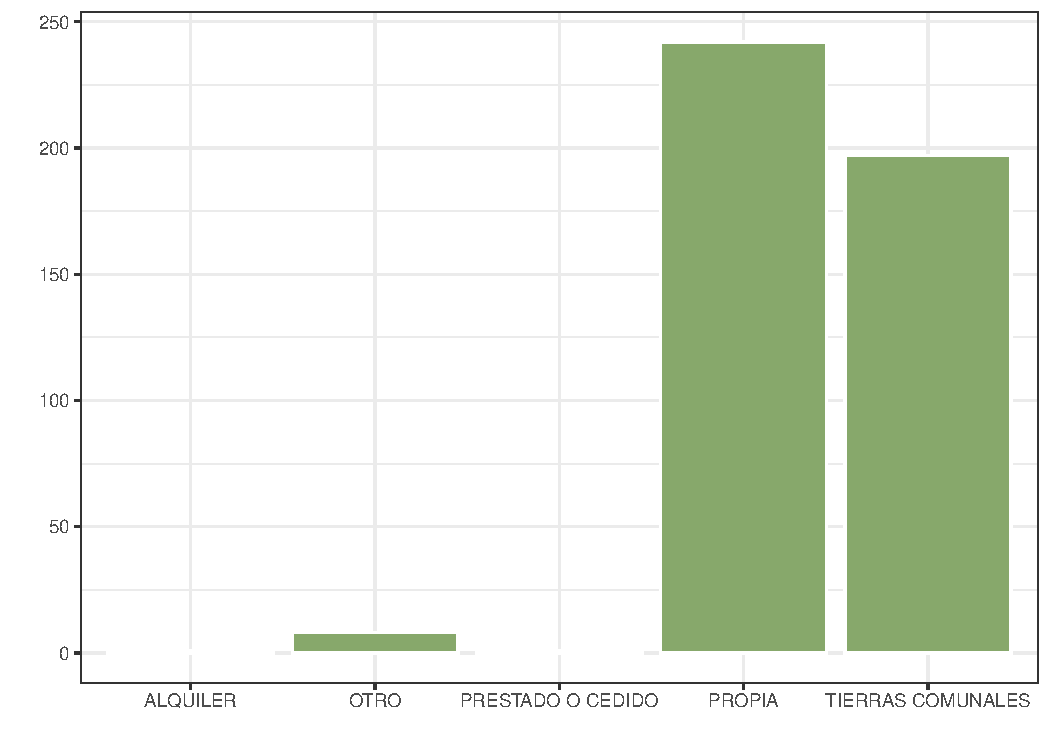
\includegraphics[width=\maxwidth]{figure/fig_dieciseis-1} 
\end{knitrout}
}
\end{graficas}

\begin{fotos}
{aplicacion de encuestas}{14}
\end{fotos}


\begin{tablas}
{Tipo de documento de la parcela}{

\begin{tabular}{lcl}
\toprule
\cellcolor[HTML]{87A96B}{\textcolor{black}{\textbf{Documento\_parcela}}} & \cellcolor[HTML]{87A96B}{\textcolor{black}{\textbf{Conteo}}} & \cellcolor[HTML]{87A96B}{\textcolor{black}{\textbf{Porcentaje}}}\\
\midrule
HERENCIA & 41 & 9.19\\
OTRO & 31 & 6.95\\
POSESIONARIO & 139 & 31.17\\
TITULO COMUNAL & 200 & 44.84\\
TITULO PROPIO & 35 & 7.85\\
\bottomrule
\end{tabular}

}
\end{tablas}

\begin{graficas}
{Tipo de documento de la parcela}{
\begin{knitrout}
\definecolor{shadecolor}{rgb}{0.969, 0.969, 0.969}\color{fgcolor}
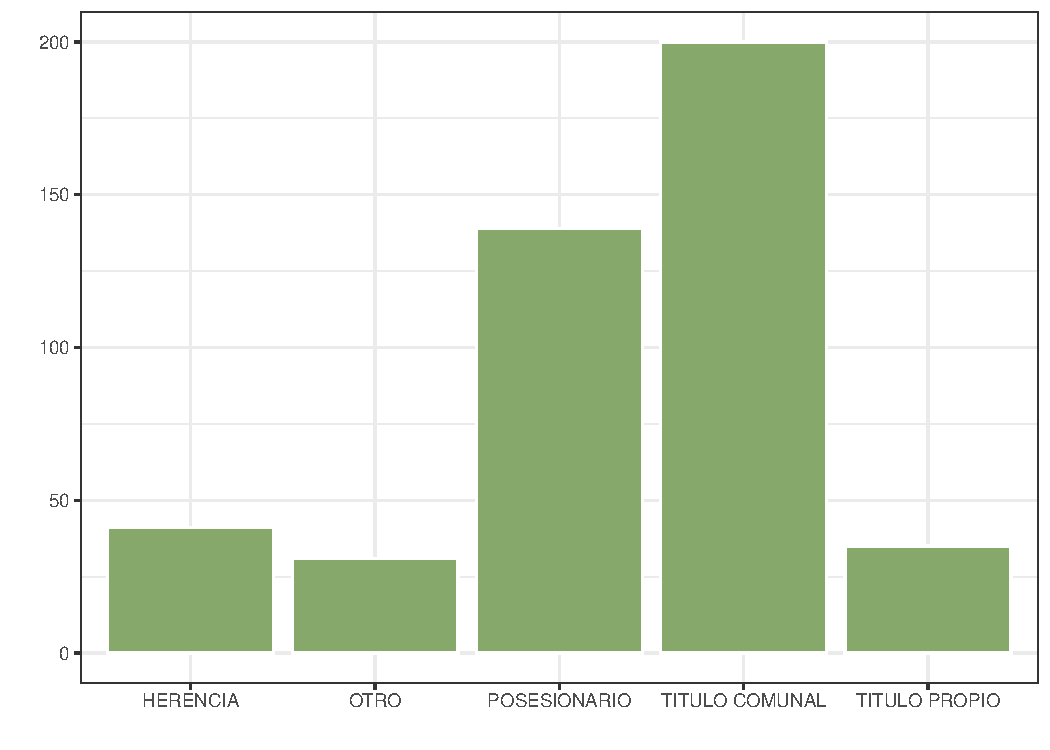
\includegraphics[width=\maxwidth]{figure/fig_diesiete-1} 
\end{knitrout}
}
\end{graficas}

\begin{fotos}
{reconocimiento en campo}{15}
\end{fotos}


\begin{tablas}
{Organizacion a la que pertenece}{

\begin{tabular}{lcl}
\toprule
\cellcolor[HTML]{87A96B}{\textcolor{black}{\textbf{Tipo\_organizacion}}} & \cellcolor[HTML]{87A96B}{\textcolor{black}{\textbf{Conteo}}} & \cellcolor[HTML]{87A96B}{\textcolor{black}{\textbf{Porcentaje}}}\\
\midrule
COMISION DE REGANTES & 201 & 45.48\\
COMITE DE USUARIOS & 171 & 38.69\\
JUNTA DE USUARIOS & 70 & 15.84\\
\bottomrule
\end{tabular}


}
\end{tablas}

\begin{graficas}
{Organizacion a la que pertenece}{
\begin{knitrout}
\definecolor{shadecolor}{rgb}{0.969, 0.969, 0.969}\color{fgcolor}
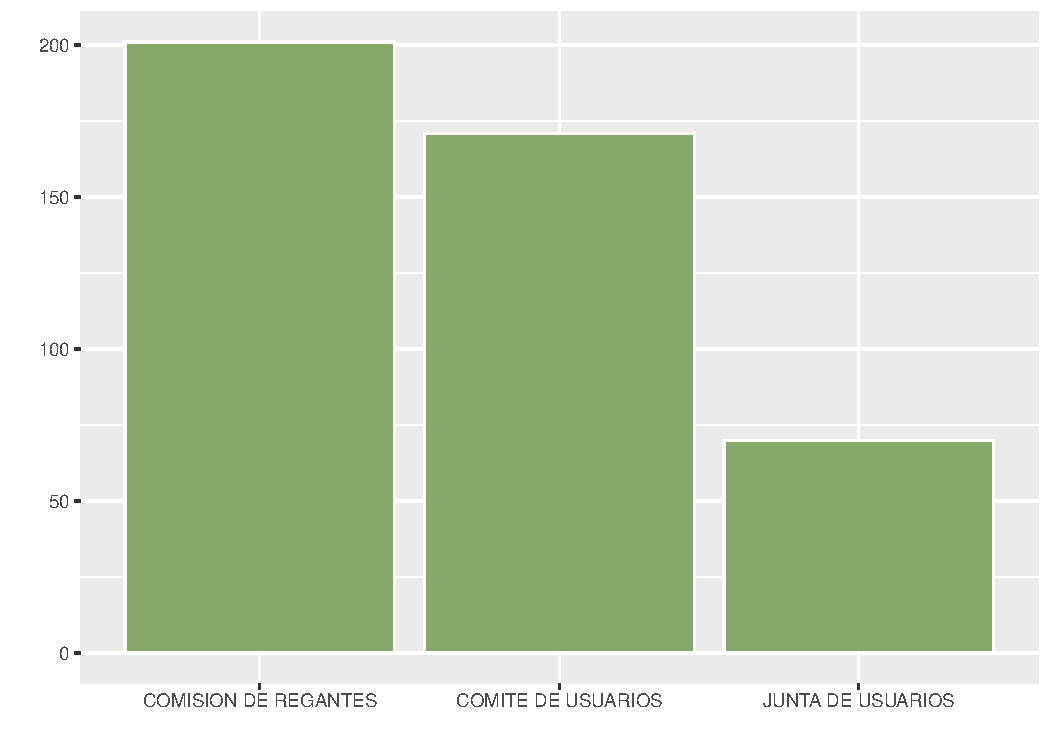
\includegraphics[width=\maxwidth]{figure/fig_dieciocho-1} 
\end{knitrout}
}
\end{graficas}

\begin{fotos}
{reconocimiento en campo}{16}
\end{fotos}

\begin{comment}
\begin{tablas}
{Organizacion a la que pertenece}{

\begin{tabular}{lcl}
\toprule
\cellcolor[HTML]{87A96B}{\textcolor{black}{\textbf{Tiempo\_organizacion}}} & \cellcolor[HTML]{87A96B}{\textcolor{black}{\textbf{Conteo}}} & \cellcolor[HTML]{87A96B}{\textcolor{black}{\textbf{Porcentaje}}}\\
\midrule
0.5 H & 1 & 0.27\\
05 A & 1 & 0.27\\
1 A & 5 & 1.36\\
1 AÑO & 2 & 0.54\\
1 TOPO & 1 & 0.27\\
\addlinespace
1/2 TOPO & 1 & 0.27\\
10 & 17 & 4.62\\
10 A & 8 & 2.17\\
10 AÑOS & 19 & 5.16\\
10 AÑOS & 2 & 0.54\\
\addlinespace
11 AÑOS & 2 & 0.54\\
11 AÑOS & 1 & 0.27\\
12 & 1 & 0.27\\
12 A & 5 & 1.36\\
12 AÑOS & 4 & 1.09\\
\addlinespace
12 AÑOS & 1 & 0.27\\
13 A & 2 & 0.54\\
13 AÑOS & 5 & 1.36\\
14 & 1 & 0.27\\
14 A & 3 & 0.82\\
\addlinespace
15 & 20 & 5.43\\
15 A & 4 & 1.09\\
15 AÑ0S & 1 & 0.27\\
15 AÑOS & 25 & 6.79\\
15 AÑOS & 2 & 0.54\\
\addlinespace
16 AÑOS & 1 & \vphantom{1} 0.27\\
17 & 1 & 0.27\\
17 A & 2 & 0.54\\
17 AÑOS & 1 & 0.27\\
18 & 2 & 0.54\\
\addlinespace
18 A & 16 & 4.35\\
18 AÑOS & 4 & 1.09\\
18 AÑOS & 1 & 0.27\\
19 AÑOS & 1 & 0.27\\
2 A & 3 & 0.82\\
\addlinespace
2 AÑOS & 8 & 2.17\\
20 & 4 & 1.09\\
20 A & 9 & 2.45\\
20 AÑOS & 22 & 5.98\\
20 AÑOS & 3 & 0.82\\
\addlinespace
22 & 1 & 0.27\\
22 A & 3 & 0.82\\
23 A & 3 & 0.82\\
24 A & 2 & 0.54\\
24 AÑOS & 8 & 2.17\\
\addlinespace
25 & 1 & 0.27\\
25 A & 8 & 2.17\\
25 AÑOS & 5 & 1.36\\
25 HA & 1 & 0.27\\
25 años & 1 & 0.27\\
\addlinespace
27 A & 1 & 0.27\\
27 AÑOS & 1 & 0.27\\
28 & 1 & 0.27\\
3 A & 12 & 3.26\\
3 AÑOS & 3 & 0.82\\
\addlinespace
30 & 1 & 0.27\\
30 A & 6 & 1.63\\
30 AÑOS & 8 & 2.17\\
31 A & 1 & 0.27\\
35 AÑOS & 1 & 0.27\\
\addlinespace
36 A & 1 & 0.27\\
39 A & 2 & 0.54\\
4 A & 7 & 1.90\\
4 AÑOS & 4 & 1.09\\
40 & 3 & 0.82\\
\addlinespace
40 A & 2 & 0.54\\
40 AÑOS & 9 & 2.45\\
40 AÑOS & 1 & 0.27\\
45 A & 1 & 0.27\\
45 AÑOS & 1 & 0.27\\
\addlinespace
5 & 2 & 0.54\\
5 A & 4 & 1.09\\
5 AÑOS & 7 & 1.90\\
5 AÑOS & 1 & 0.27\\
50 A & 1 & 0.27\\
\addlinespace
50 AÑOS & 2 & 0.54\\
6 & 1 & 0.27\\
6 AÑOS & 1 & 0.27\\
6 AÑOS & 1 & 0.27\\
60 A & 1 & 0.27\\
\addlinespace
60 AÑOS & 3 & 0.82\\
7 & 1 & 0.27\\
7 A & 2 & 0.54\\
70 AÑOS & 1 & 0.27\\
8 & 2 & 0.54\\
\addlinespace
8 A & 14 & 3.80\\
8 AÑOS & 2 & 0.54\\
DESDE SIEMPRE & 1 & 0.27\\
MAS DE 12 A & 1 & 0.27\\
MAS DE 15 AÑOS & 8 & 2.17\\
\addlinespace
MAS DE 20 AÑOS & 1 & 0.27\\
\bottomrule
\end{tabular}


}
\end{tablas}

\begin{graficas}
{Organizacion a la que pertenece}{
\begin{knitrout}
\definecolor{shadecolor}{rgb}{0.969, 0.969, 0.969}\color{fgcolor}
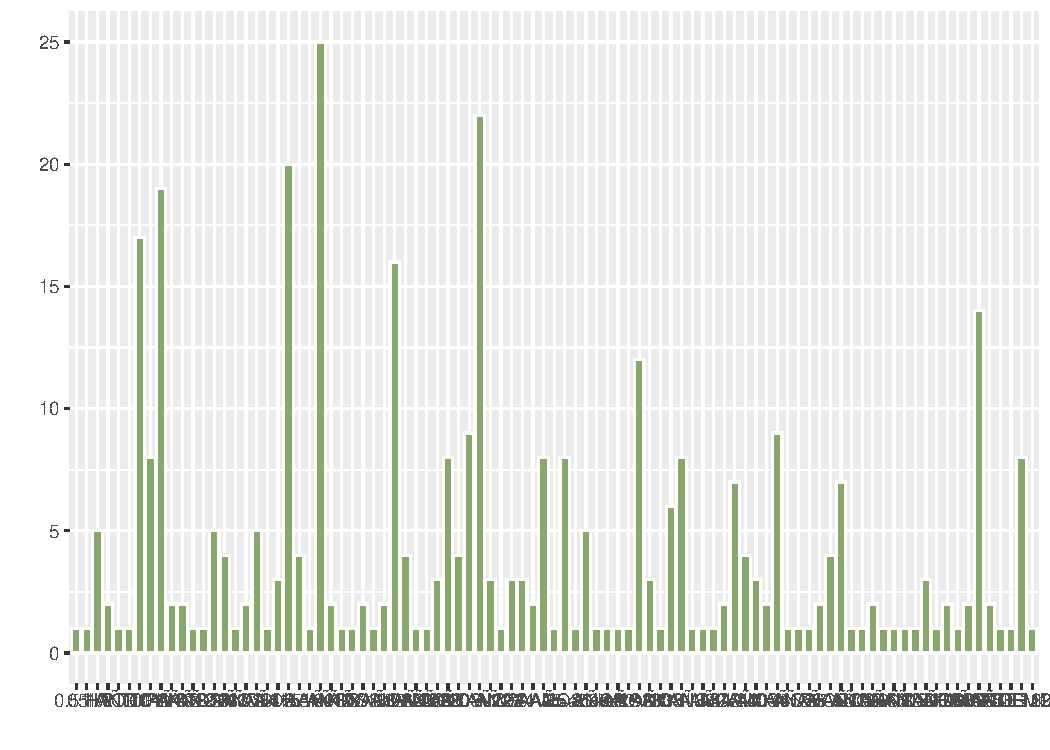
\includegraphics[width=\maxwidth]{figure/fig_diecinueve-1} 
\end{knitrout}
}
\end{graficas}

%\begin{fotos}
%{reconocimiento en campo}{17}
%\end{fotos}
\end{comment}

\begin{tablas}
{Fuente del agua para riego}{

\begin{tabular}{lcl}
\toprule
\cellcolor[HTML]{87A96B}{\textcolor{black}{\textbf{Fuente\_riego}}} & \cellcolor[HTML]{87A96B}{\textcolor{black}{\textbf{Conteo}}} & \cellcolor[HTML]{87A96B}{\textcolor{black}{\textbf{Porcentaje}}}\\
\midrule
LAGO O LAGUNA & 2 & 0.45\\
MANANTIAL & 217 & 48.55\\
OTRO & 18 & 4.03\\
POZOS & 1 & 0.22\\
RIO & 209 & 46.76\\
\bottomrule
\end{tabular}


}
\end{tablas}
\begin{graficas}
{Fuente del agua para riego}{
\begin{knitrout}
\definecolor{shadecolor}{rgb}{0.969, 0.969, 0.969}\color{fgcolor}
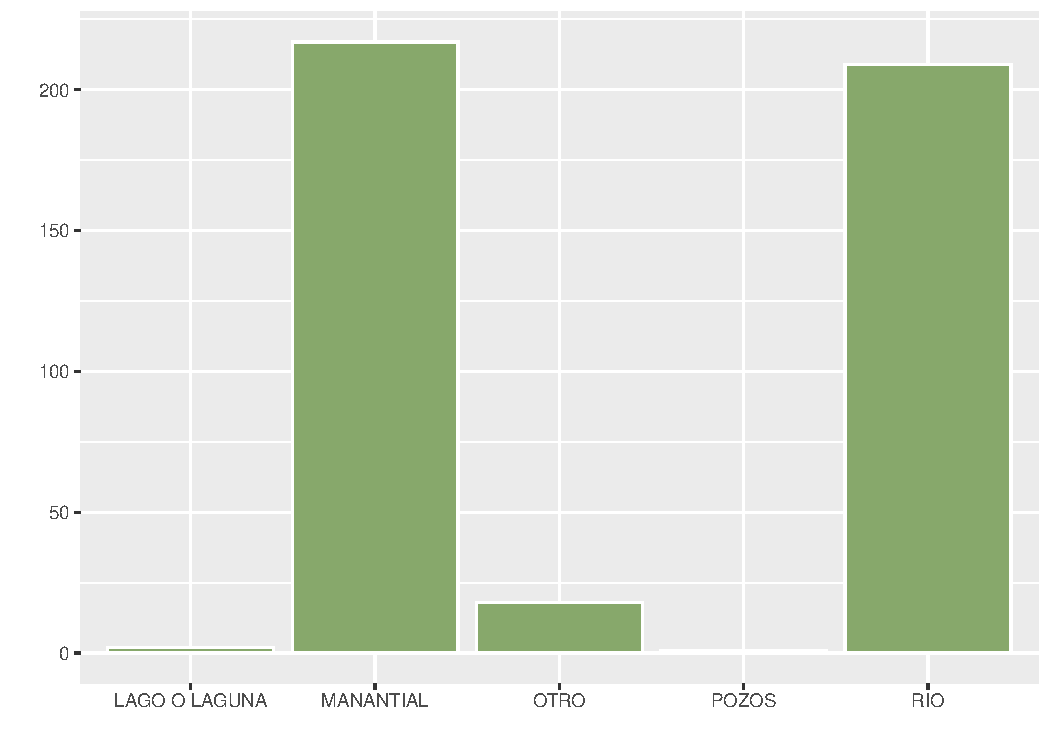
\includegraphics[width=\maxwidth]{figure/fig_veinte-1} 
\end{knitrout}
}
\end{graficas}
\begin{fotos}
{reconocimiento en campo}{18}
\end{fotos}

\begin{comment}
\begin{tablas}
{Fuente de agua para riego}{

\begin{tabular}{lcl}
\toprule
\cellcolor[HTML]{87A96B}{\textcolor{black}{\textbf{Fuente\_riego}}} & \cellcolor[HTML]{87A96B}{\textcolor{black}{\textbf{Conteo}}} & \cellcolor[HTML]{87A96B}{\textcolor{black}{\textbf{Porcentaje}}}\\
\midrule
LAGO O LAGUNA & 2 & 0.45\\
MANANTIAL & 217 & 48.55\\
OTRO & 18 & 4.03\\
POZOS & 1 & 0.22\\
RIO & 209 & 46.76\\
\bottomrule
\end{tabular}


}
\end{tablas}
\begin{graficas}
{Fuente de agua para riego}{
\begin{knitrout}
\definecolor{shadecolor}{rgb}{0.969, 0.969, 0.969}\color{fgcolor}
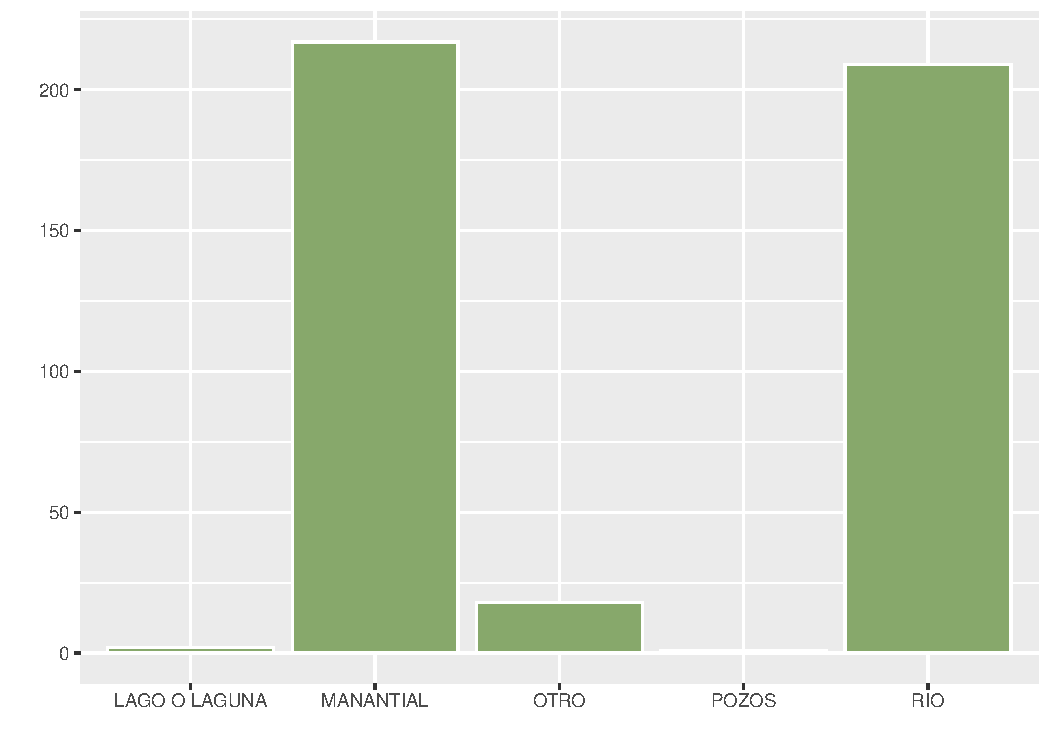
\includegraphics[width=\maxwidth]{figure/fig_veintiuno-1} 
\end{knitrout}
}
\end{graficas}
%\begin{fotos}
%{reconocimiento en campo}{19}
%\end{fotos}
\end{comment}

\begin{tablas}
{Frecuencia de riego de la parcela}{

\begin{tabular}{lcl}
\toprule
\cellcolor[HTML]{87A96B}{\textcolor{black}{\textbf{Frecuencia\_riego}}} & \cellcolor[HTML]{87A96B}{\textcolor{black}{\textbf{Conteo}}} & \cellcolor[HTML]{87A96B}{\textcolor{black}{\textbf{Porcentaje}}}\\
\midrule
OTRO & 31 & 7.01\\
POR DIAS & 83 & 18.78\\
POR HORAS & 20 & 4.52\\
POR TURNOS & 305 & 69.00\\
POR VOLUMEN & 3 & 0.68\\
\bottomrule
\end{tabular}


}
\end{tablas}
\begin{graficas}
{Frecuencia de riego de la parcela}{
\begin{knitrout}
\definecolor{shadecolor}{rgb}{0.969, 0.969, 0.969}\color{fgcolor}
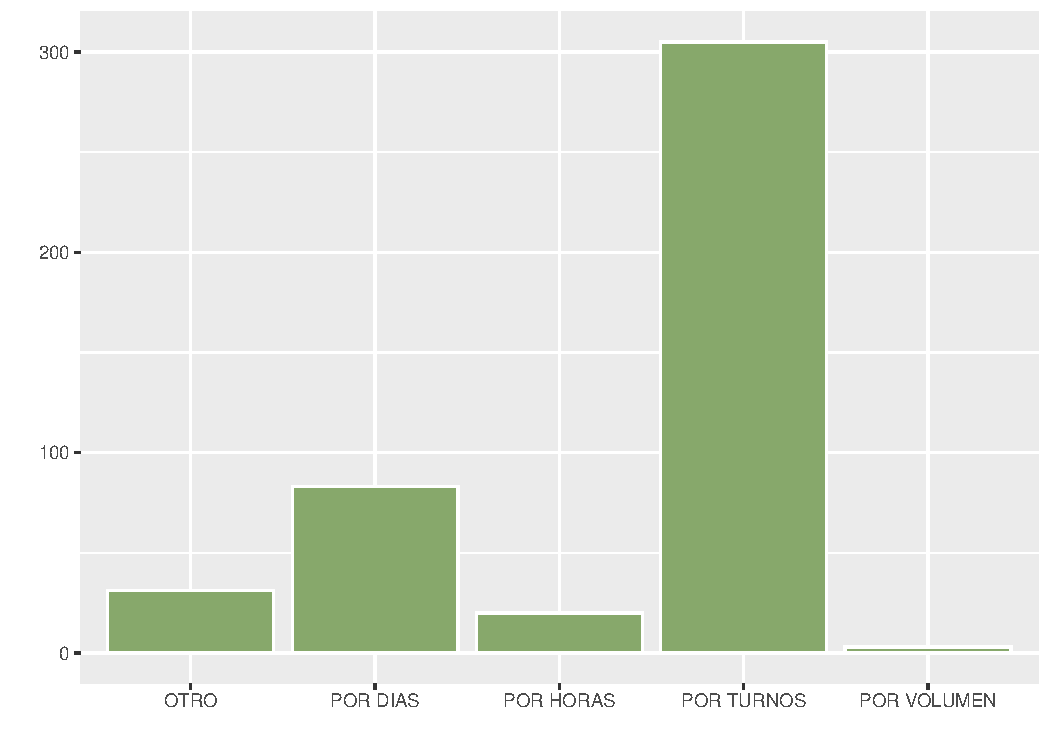
\includegraphics[width=\maxwidth]{figure/fig_veintidos-1} 
\end{knitrout}
}
\end{graficas}
\begin{fotos}
{reconocimiento en campo}{20}
\end{fotos}

\begin{tablas}
{Infraestructura de riego}{

\begin{tabular}{lcl}
\toprule
\cellcolor[HTML]{87A96B}{\textcolor{black}{\textbf{Tipo\_infraestructura}}} & \cellcolor[HTML]{87A96B}{\textcolor{black}{\textbf{Conteo}}} & \cellcolor[HTML]{87A96B}{\textcolor{black}{\textbf{Porcentaje}}}\\
\midrule
REBESTIDO & 259 & 72.35\\
TAJO ABIERTO & 99 & 27.65\\
\bottomrule
\end{tabular}


}
\end{tablas}
\begin{graficas}
{Infraestructura de riego}{
\begin{knitrout}
\definecolor{shadecolor}{rgb}{0.969, 0.969, 0.969}\color{fgcolor}
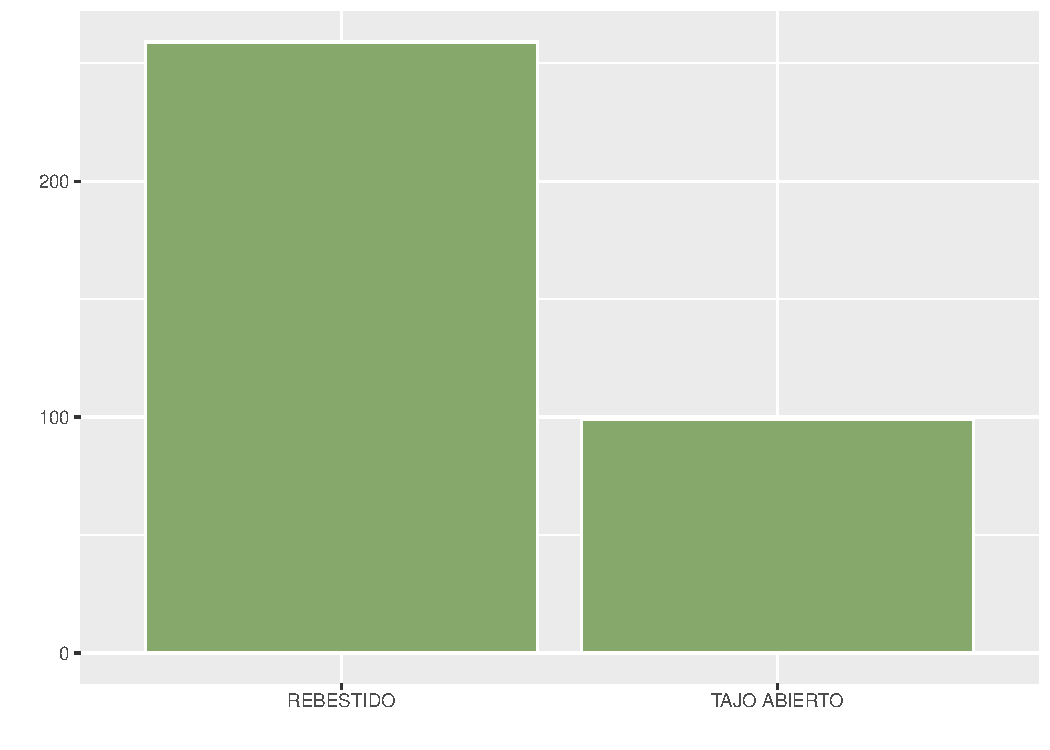
\includegraphics[width=\maxwidth]{figure/fig_veintitres-1} 
\end{knitrout}
}
\end{graficas}
\begin{fotos}
{reconocimiento en campo}{21}
\end{fotos}


\begin{tablas}
{Tipo de riego que utiliza}{

\begin{tabular}{lcl}
\toprule
\cellcolor[HTML]{87A96B}{\textcolor{black}{\textbf{Tipo\_riego}}} & \cellcolor[HTML]{87A96B}{\textcolor{black}{\textbf{Conteo}}} & \cellcolor[HTML]{87A96B}{\textcolor{black}{\textbf{Porcentaje}}}\\
\midrule
OTRO & 9 & 2.04\\
POR GRAVEDAD & 43 & 9.73\\
POZO O AGUA SUBTERRANEA & 1 & 0.23\\
TECNIFICADO & 389 & 88.01\\
\bottomrule
\end{tabular}


}
\end{tablas}
\begin{graficas}
{Tipo de riego que utiliza}{
\begin{knitrout}
\definecolor{shadecolor}{rgb}{0.969, 0.969, 0.969}\color{fgcolor}
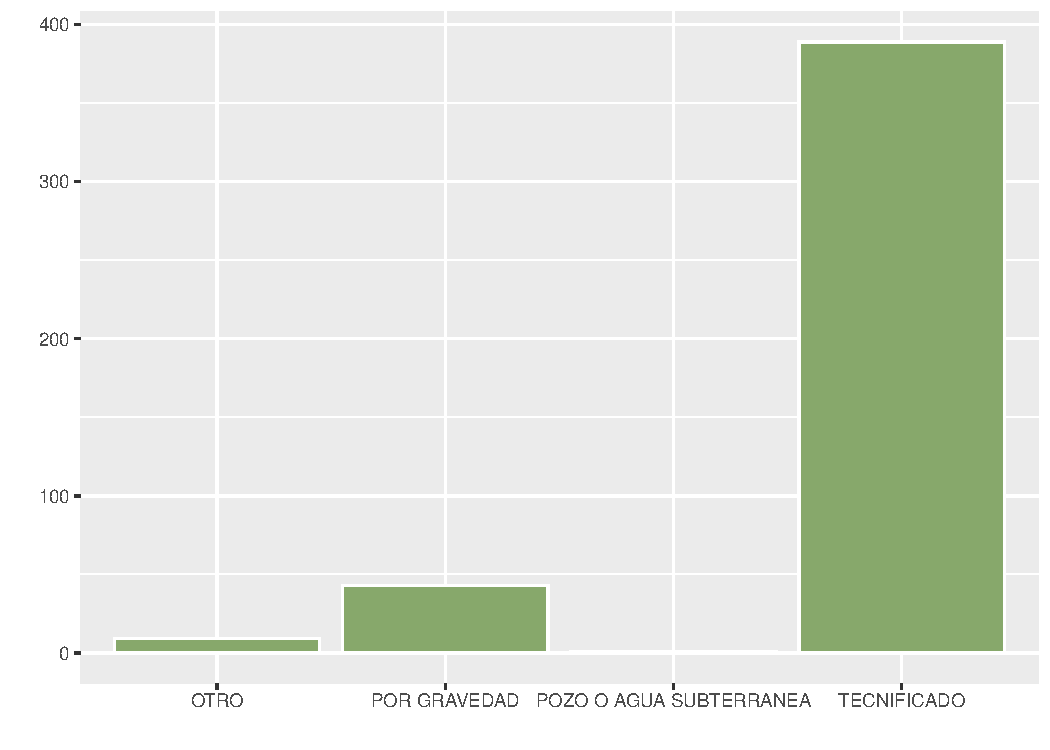
\includegraphics[width=\maxwidth]{figure/fig_veinticuatro-1} 
\end{knitrout}
}
\end{graficas}
\begin{fotos}
{reconocimiento en campo}{22}
\end{fotos}


\begin{tablas}
{Pago por uso de agua para riego}{

\begin{tabular}{lcl}
\toprule
\cellcolor[HTML]{87A96B}{\textcolor{black}{\textbf{Pago\_agua}}} & \cellcolor[HTML]{87A96B}{\textcolor{black}{\textbf{Conteo}}} & \cellcolor[HTML]{87A96B}{\textcolor{black}{\textbf{Porcentaje}}}\\
\midrule
NO & 27 & 6.15\\
SI & 412 & 93.85\\
\bottomrule
\end{tabular}


}
\end{tablas}
\begin{graficas}
{Pago por uso de agua para riego}{
\begin{knitrout}
\definecolor{shadecolor}{rgb}{0.969, 0.969, 0.969}\color{fgcolor}
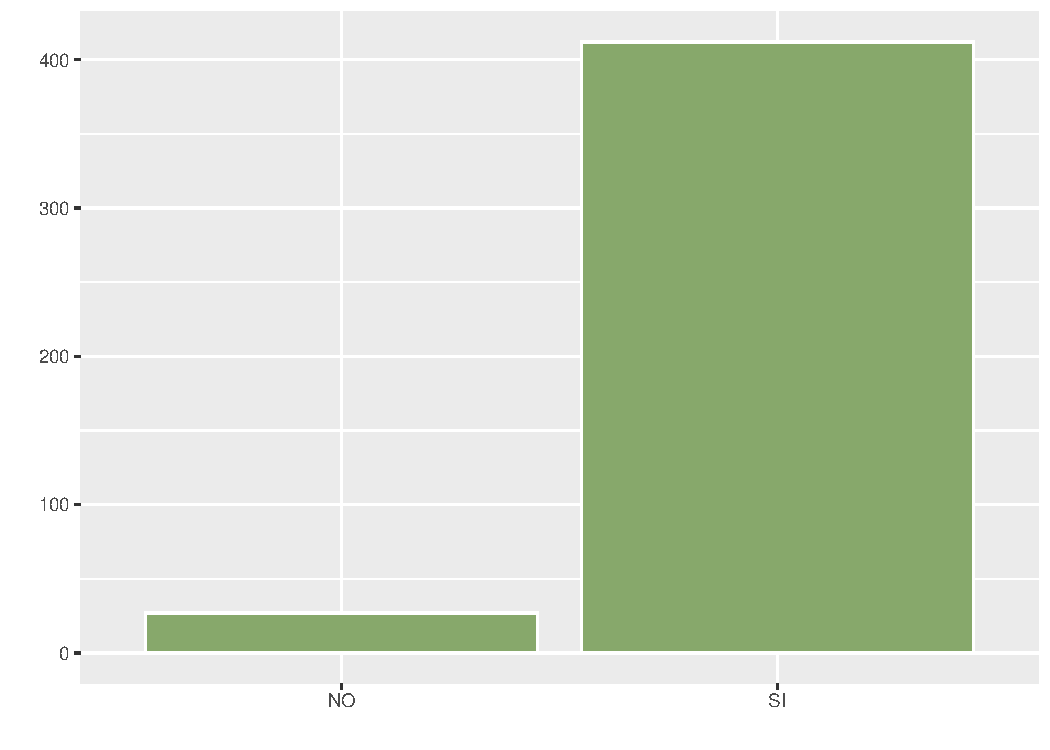
\includegraphics[width=\maxwidth]{figure/fig_veinticinco-1} 
\end{knitrout}
}
\end{graficas}
\begin{fotos}
{reconocimiento en campo}{23}
\end{fotos}


\begin{tablas}
{Frecuencia por uso de agua para riego}{

\begin{tabular}{lcl}
\toprule
\cellcolor[HTML]{87A96B}{\textcolor{black}{\textbf{Frecuencia\_pago}}} & \cellcolor[HTML]{87A96B}{\textcolor{black}{\textbf{Conteo}}} & \cellcolor[HTML]{87A96B}{\textcolor{black}{\textbf{Porcentaje}}}\\
\midrule
ANUAL & 348 & 85.93\\
DIARIO & 24 & 5.93\\
MENSUAL & 18 & 4.44\\
QUINCENAL & 6 & 1.48\\
SEMESTRAL & 9 & 2.22\\
\bottomrule
\end{tabular}


}
\end{tablas}
\begin{graficas}
{Frecuencia por uso de agua para riego}{
\begin{knitrout}
\definecolor{shadecolor}{rgb}{0.969, 0.969, 0.969}\color{fgcolor}
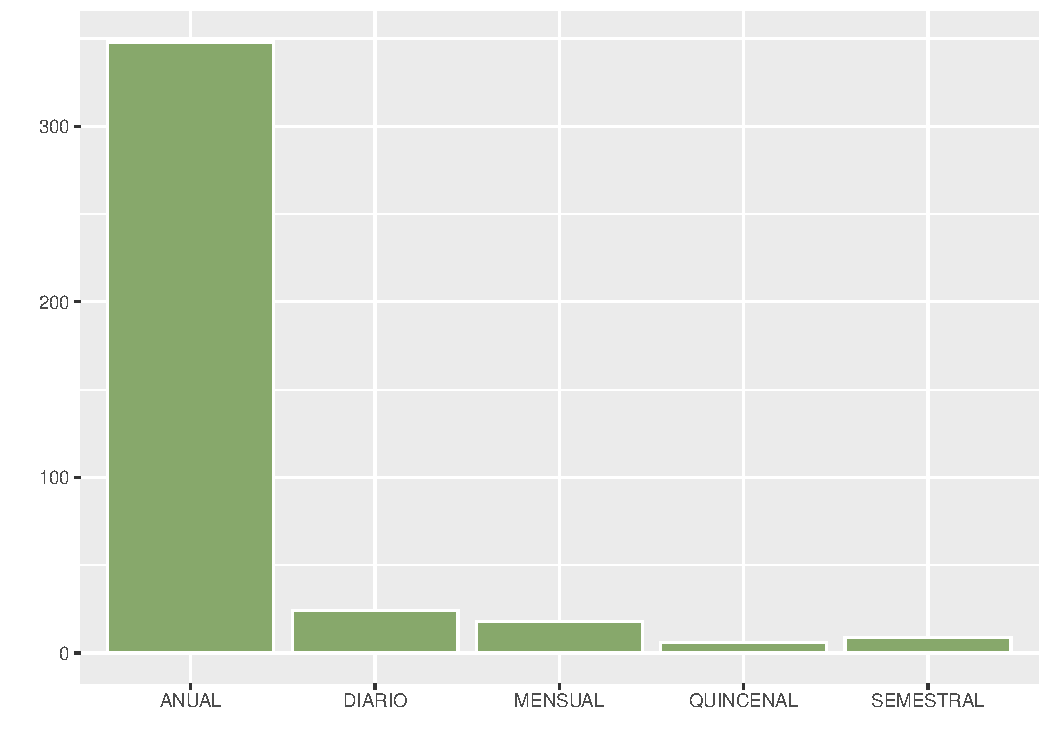
\includegraphics[width=\maxwidth]{figure/fig_veintiseis-1} 
\end{knitrout}
}
\end{graficas}
\begin{fotos}
{reconocimiento en campo}{24}
\end{fotos}


\begin{tablas}
{Derecho de uso de agua}{

\begin{tabular}{lcl}
\toprule
\cellcolor[HTML]{87A96B}{\textcolor{black}{\textbf{Derecho}}} & \cellcolor[HTML]{87A96B}{\textcolor{black}{\textbf{Conteo}}} & \cellcolor[HTML]{87A96B}{\textcolor{black}{\textbf{Porcentaje}}}\\
\midrule
NO & 6 & 1.36\\
SI & 434 & 98.64\\
\bottomrule
\end{tabular}


}
\end{tablas}
\begin{graficas}
{Derecho de uso de agua}{
\begin{knitrout}
\definecolor{shadecolor}{rgb}{0.969, 0.969, 0.969}\color{fgcolor}
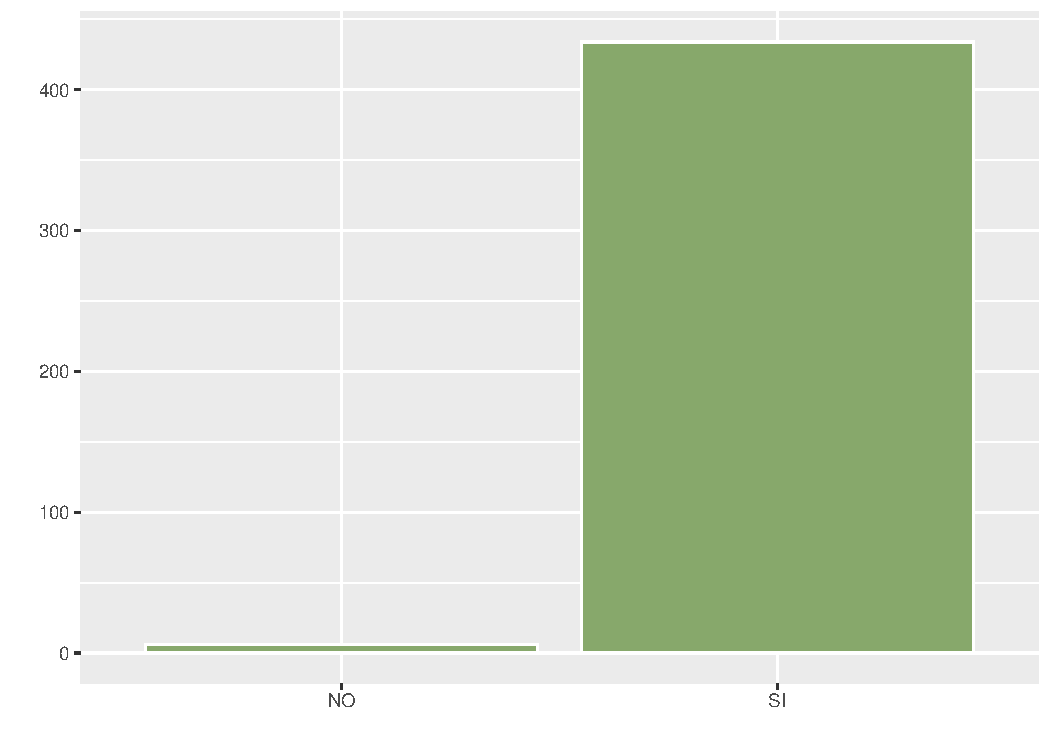
\includegraphics[width=\maxwidth]{figure/fig_veintisiete-1} 
\end{knitrout}
}
\end{graficas}
\begin{fotos}
{aplicacion de encuesta}{25}
\end{fotos}


\begin{tablas}
{Produccion predominante}{

\begin{tabular}{lcl}
\toprule
\cellcolor[HTML]{87A96B}{\textcolor{black}{\textbf{Cultivo}}} & \cellcolor[HTML]{87A96B}{\textcolor{black}{\textbf{Conteo}}} & \cellcolor[HTML]{87A96B}{\textcolor{black}{\textbf{Porcentaje}}}\\
\midrule
HORTALIZAS & 9 & 2.03\\
MAIZ CHOCLO & 40 & 9.03\\
MAIZ CHOCLO, HORTALIZAS & 7 & 1.58\\
MAIZ CHOCLO, HORTALIZAS, OTRO & 1 & 0.23\\
MAIZ CHOCLO, OTRO & 2 & 0.45\\
\addlinespace
OTRO & 2 & 0.45\\
PAPA & 12 & 2.71\\
PAPA, HORTALIZAS & 1 & 0.23\\
PAPA, MAIZ CHOCLO & 47 & 10.61\\
PAPA, MAIZ CHOCLO, HORTALIZAS & 10 & 2.26\\
\addlinespace
PAPA, MAIZ CHOCLO, HORTALIZAS, OTRO & 1 & 0.23\\
PAPA, MAIZ CHOCLO, OTRO & 1 & 0.23\\
PAPA, OTRO & 1 & 0.23\\
PASTOS & 60 & 13.54\\
PASTOS, HORTALIZAS & 1 & 0.23\\
\addlinespace
PASTOS, MAIZ CHOCLO & 5 & 1.13\\
PASTOS, MAIZ CHOCLO, HORTALIZAS & 1 & 0.23\\
PASTOS, PAPA & 7 & 1.58\\
PASTOS, PAPA, HORTALIZAS & 27 & 6.09\\
PASTOS, PAPA, HORTALIZAS, OTRO & 4 & 0.90\\
\addlinespace
PASTOS, PAPA, MAIZ CHOCLO & 50 & 11.29\\
PASTOS, PAPA, MAIZ CHOCLO, HORTALIZAS & 141 & 31.83\\
PASTOS, PAPA, MAIZ CHOCLO, HORTALIZAS, OTRO & 5 & 1.13\\
PASTOS, PAPA, MAIZ CHOCLO, OTRO & 4 & 0.90\\
PASTOS, PAPA, OTRO & 4 & 0.90\\
\bottomrule
\end{tabular}


}
\end{tablas}

\begin{graficas}
{Produccion predominante}{
\begin{knitrout}
\definecolor{shadecolor}{rgb}{0.969, 0.969, 0.969}\color{fgcolor}
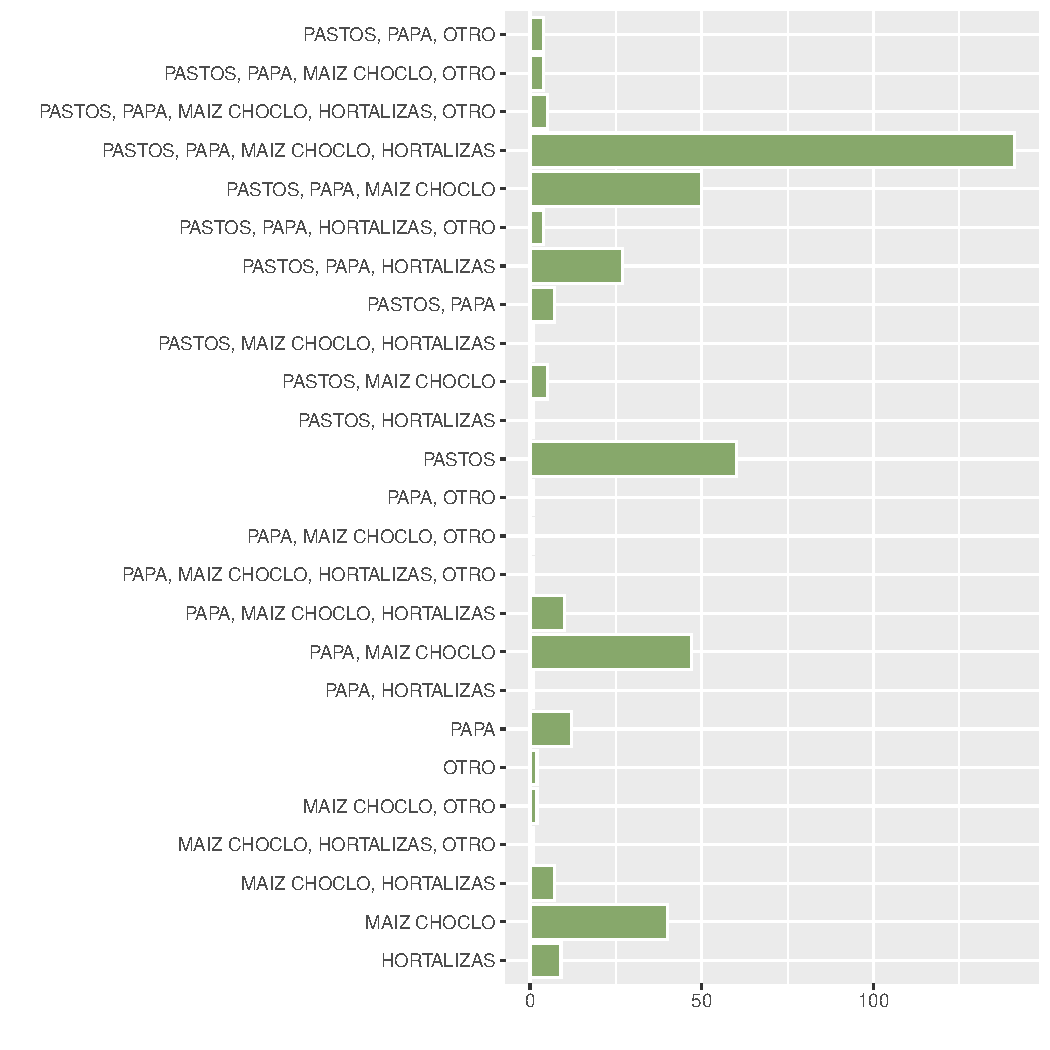
\includegraphics[width=\maxwidth]{figure/fig_veintiocho-1} 
\end{knitrout}
}
\end{graficas}

\begin{fotos}
{aplicacion de encuesta}{26}
\end{fotos}


\begin{tablas}
{Tiempo que se dedica al cultivo}{

\begin{tabular}{lcl}
\toprule
\cellcolor[HTML]{87A96B}{\textcolor{black}{\textbf{Tiempo}}} & \cellcolor[HTML]{87A96B}{\textcolor{black}{\textbf{Conteo}}} & \cellcolor[HTML]{87A96B}{\textcolor{black}{\textbf{Porcentaje}}}\\
\midrule
HACE 02 AÑOS & 3 & 0.71\\
HACE 1 AÑO & 3 & 0.71\\
MAS DE 3 AÑOS & 56 & 13.30\\
MAS DE 5 AÑOS & 359 & 85.27\\
\bottomrule
\end{tabular}


}
\end{tablas}

\begin{graficas}
{Tiempo que se dedica al cultivo}{
\begin{knitrout}
\definecolor{shadecolor}{rgb}{0.969, 0.969, 0.969}\color{fgcolor}
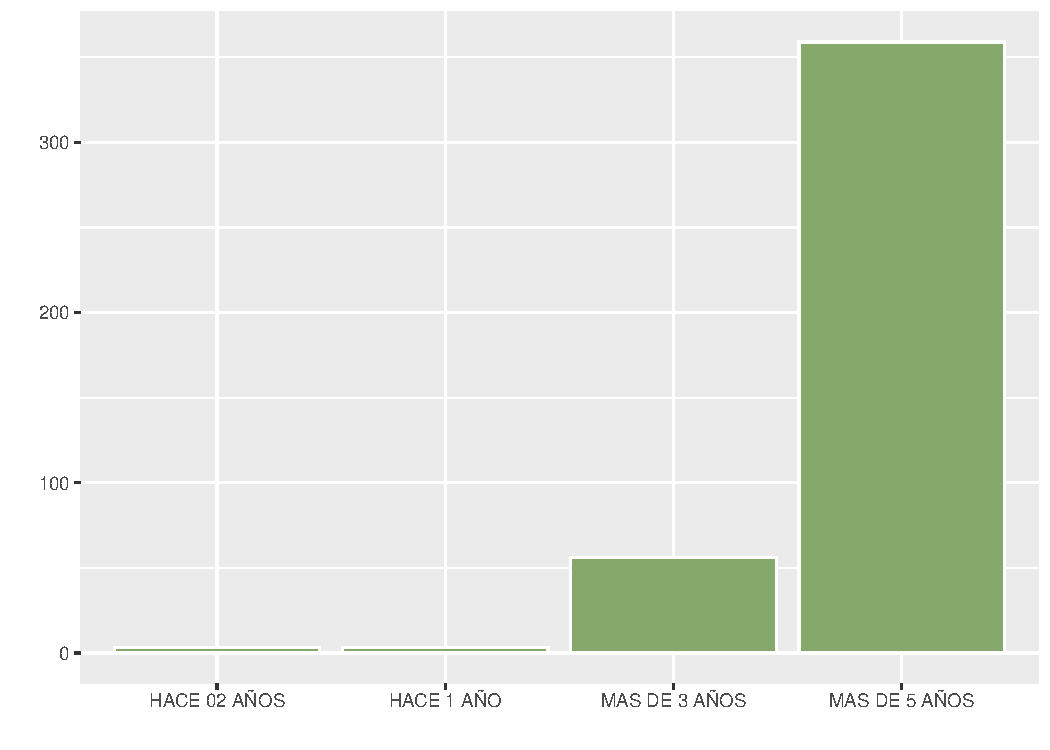
\includegraphics[width=\maxwidth]{figure/fig_veintinueve-1} 
\end{knitrout}
}
\end{graficas}

\begin{fotos}
{socializacion del proyecto}{27}
\end{fotos}


\begin{tablas}
{Finalidad de cosecha}{

\begin{tabular}{lcl}
\toprule
\cellcolor[HTML]{87A96B}{\textcolor{black}{\textbf{Finalidad}}} & \cellcolor[HTML]{87A96B}{\textcolor{black}{\textbf{Conteo}}} & \cellcolor[HTML]{87A96B}{\textcolor{black}{\textbf{Porcentaje}}}\\
\midrule
CONSUMO & 144 & 35.29\\
VENTA & 2 & 0.49\\
VENTA Y CONSUMO & 262 & 64.22\\
\bottomrule
\end{tabular}


}
\end{tablas}

\begin{graficas}
{Finalidad de cosecha}{
\begin{knitrout}
\definecolor{shadecolor}{rgb}{0.969, 0.969, 0.969}\color{fgcolor}
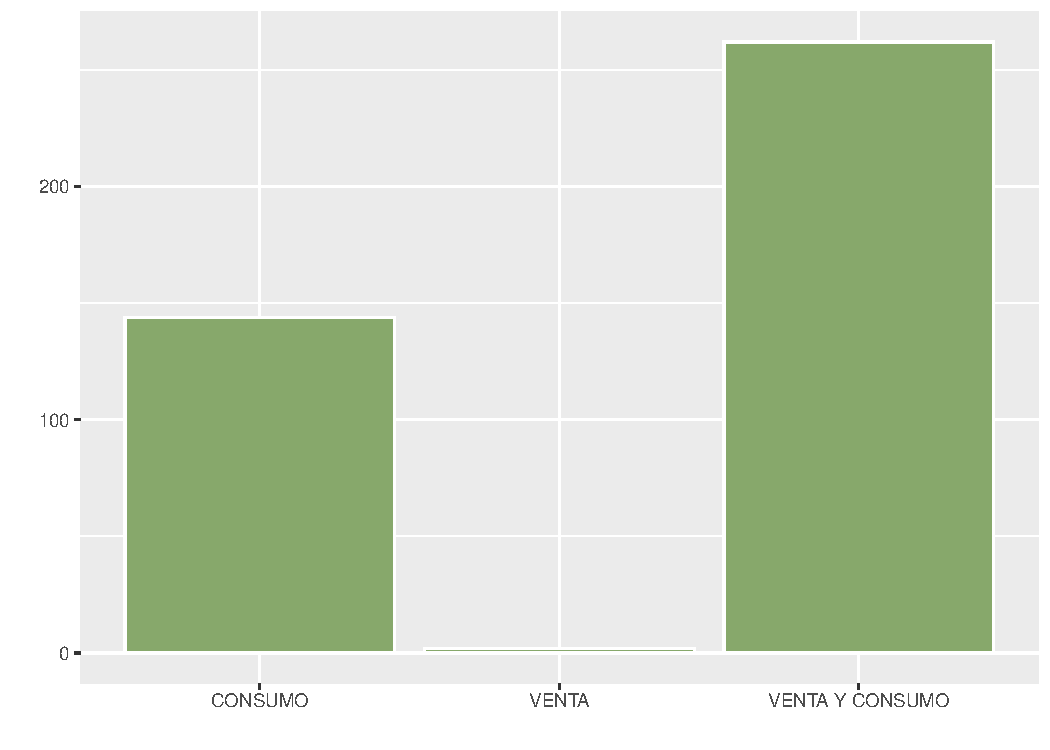
\includegraphics[width=\maxwidth]{figure/fig_treinta-1} 
\end{knitrout}
}
\end{graficas}

\begin{fotos}
{socializacion del proyecto}{28}
\end{fotos}


\begin{tablas}
{Causas que ocasionan la disminucion de la produccion de cultivo}{

\begin{tabular}{lcl}
\toprule
\cellcolor[HTML]{87A96B}{\textcolor{black}{\textbf{Causas}}} & \cellcolor[HTML]{87A96B}{\textcolor{black}{\textbf{Conteo}}} & \cellcolor[HTML]{87A96B}{\textcolor{black}{\textbf{Porcentaje}}}\\
\midrule
FACTORES ADVERSOS & 22 & 5.07\\
FALTA DE AGUA & 24 & 5.53\\
FALTA DE AGUA Y FACTORES ADVERSOS & 100 & 23.04\\
FALTA DE AGUA, FACTORES ADVERSOS Y SUELOS POBRES & 267 & 61.52\\
FALTA DE AGUA, SUELOS PROBRES Y ERIAZOS & 7 & 1.61\\
\addlinespace
SUELOS POBRES & 5 & 1.15\\
SUELOS POBRES Y FACTORES ADVERSOS & 9 & 2.07\\
\bottomrule
\end{tabular}


}
\end{tablas}

\begin{graficas}
{Causas que ocasionan la disminucion de la produccion de cultivo}{
\begin{knitrout}
\definecolor{shadecolor}{rgb}{0.969, 0.969, 0.969}\color{fgcolor}
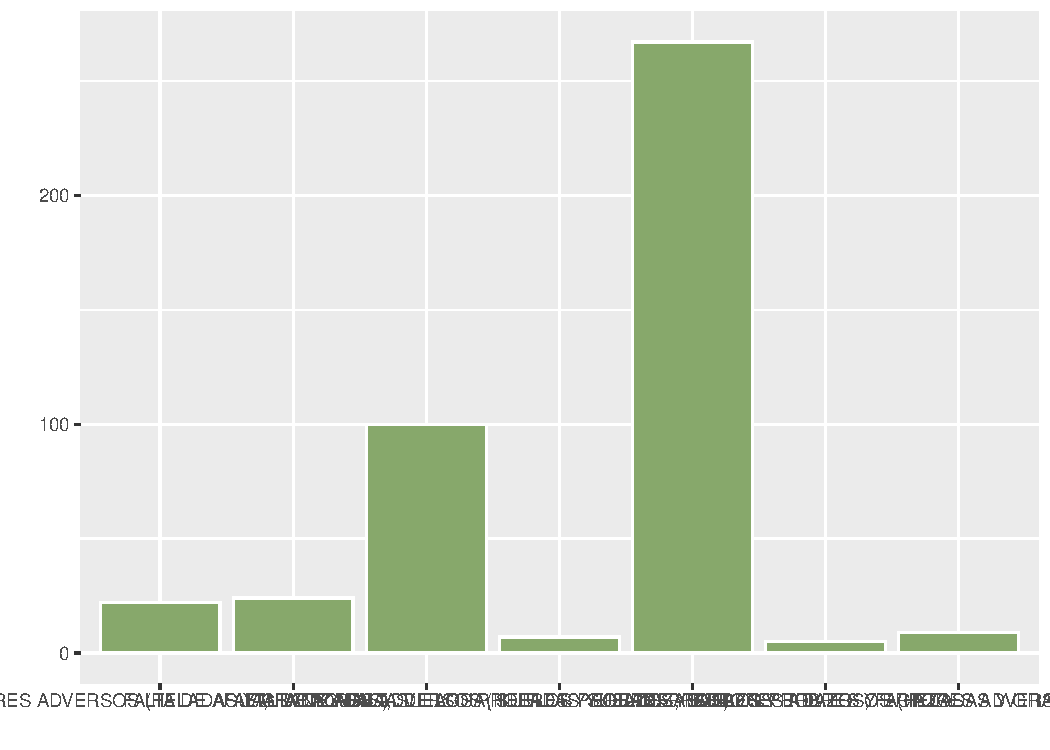
\includegraphics[width=\maxwidth]{figure/fig_treintayuno-1} 
\end{knitrout}
}
\end{graficas}

\begin{fotos}
{socializacion del proyecto}{29}
\end{fotos}

\begin{tablas}
{Registra la venta de su produccion}{

\begin{tabular}{lcl}
\toprule
\cellcolor[HTML]{87A96B}{\textcolor{black}{\textbf{Registo\_ventas}}} & \cellcolor[HTML]{87A96B}{\textcolor{black}{\textbf{Conteo}}} & \cellcolor[HTML]{87A96B}{\textcolor{black}{\textbf{Porcentaje}}}\\
\midrule
NO & 162 & 40.5\\
SI & 238 & 59.5\\
\bottomrule
\end{tabular}


}
\end{tablas}

\begin{graficas}
{Registra la venta de su produccion}{
\begin{knitrout}
\definecolor{shadecolor}{rgb}{0.969, 0.969, 0.969}\color{fgcolor}
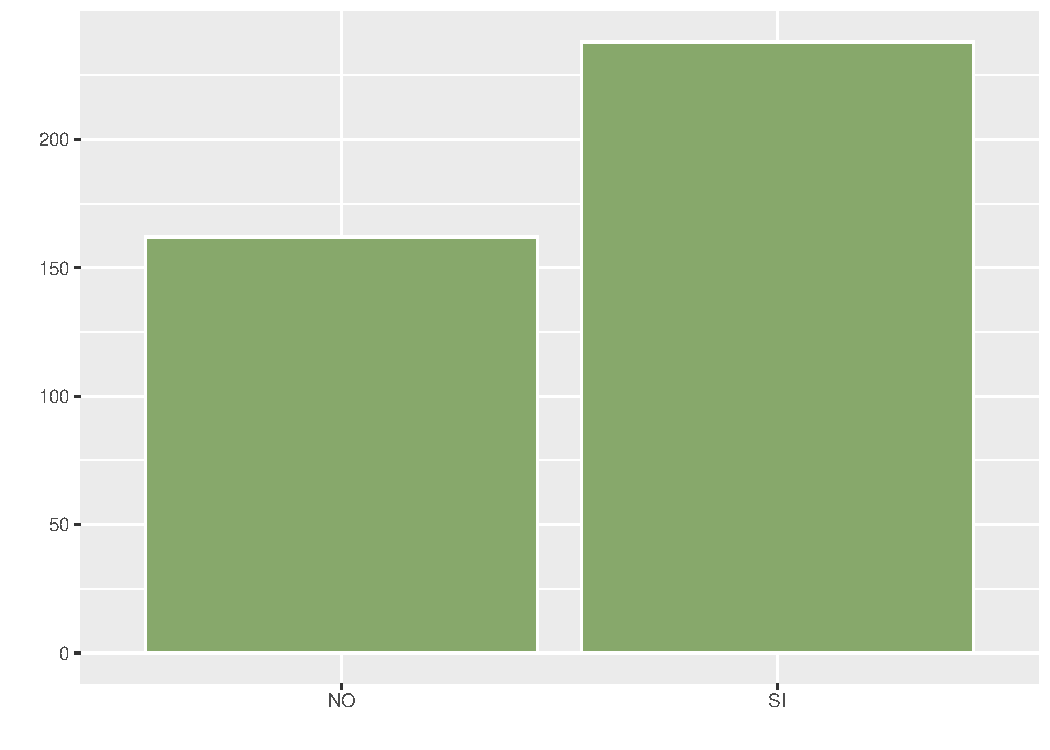
\includegraphics[width=\maxwidth]{figure/fig_treintaydos-1} 
\end{knitrout}
}
\end{graficas}

\begin{fotos}
{socializacion del proyecto}{30}
\end{fotos}

\begin{tablas}
{Personas con las que realiza la cosecha}{

\begin{tabular}{lcl}
\toprule
\cellcolor[HTML]{87A96B}{\textcolor{black}{\textbf{Personas}}} & \cellcolor[HTML]{87A96B}{\textcolor{black}{\textbf{Conteo}}} & \cellcolor[HTML]{87A96B}{\textcolor{black}{\textbf{Porcentaje}}}\\
\midrule
AMIGOS & 3 & 0.78\\
FAMILIARES & 329 & 85.01\\
JORNAL & 30 & 7.75\\
OTRO & 3 & 0.78\\
SOCIOS & 1 & 0.26\\
\addlinespace
SOLO & 21 & 5.43\\
\bottomrule
\end{tabular}


}
\end{tablas}

\begin{graficas}
{Personas con las que realiza la cosecha}{
\begin{knitrout}
\definecolor{shadecolor}{rgb}{0.969, 0.969, 0.969}\color{fgcolor}
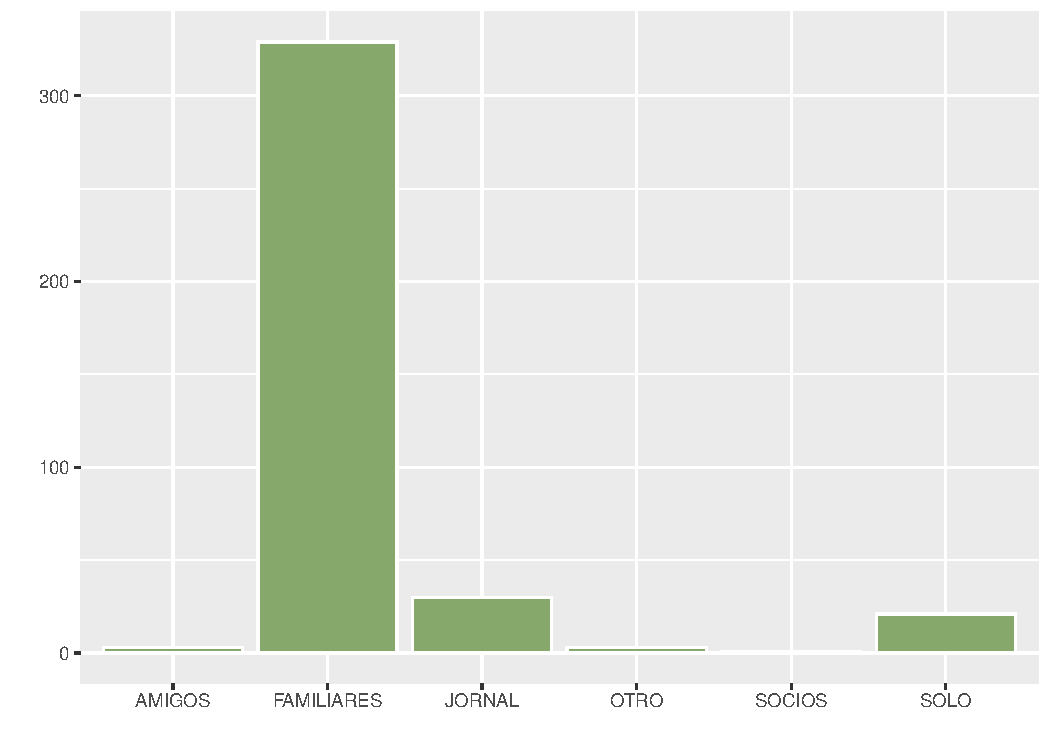
\includegraphics[width=\maxwidth]{figure/fig_treintaytres-1} 
\end{knitrout}
}
\end{graficas}

\begin{fotos}
{socializacion del proyecto}{31}
\end{fotos}


\begin{tablas}
{Practica de conservacion de suelos}{

\begin{tabular}{lcl}
\toprule
\cellcolor[HTML]{87A96B}{\textcolor{black}{\textbf{Personas}}} & \cellcolor[HTML]{87A96B}{\textcolor{black}{\textbf{Conteo}}} & \cellcolor[HTML]{87A96B}{\textcolor{black}{\textbf{Porcentaje}}}\\
\midrule
ABONOS ORGANICO Y MATERIA ORGANICA & 37 & 10.00\\
INCORPORACION EN MATERIA ORGANICA & 4 & 1.08\\
OTRO & 1 & 0.27\\
ROTACION DE CULTIVOS & 22 & 5.95\\
ROTACION DE CULTIVOS, USO DE ABONOS ORGANICOS & 129 & 34.86\\
\addlinespace
ROTACION Y MATERIA ORGANICA & 18 & 4.86\\
ROTACION, ABONO ORGANICO Y CAL & 2 & 0.54\\
ROTACION, ABONO ORGANICO, CAL Y MATERIA ORGANICA & 8 & 2.16\\
ROTACION, ABONOS ORGANICO Y MATERIA ORGANICA & 81 & 21.89\\
USO DE ABONOS ORGANICOS & 68 & 18.38\\
\bottomrule
\end{tabular}


}
\end{tablas}

\begin{graficas}
{Practica de conservacion de suelos}{
\begin{knitrout}
\definecolor{shadecolor}{rgb}{0.969, 0.969, 0.969}\color{fgcolor}
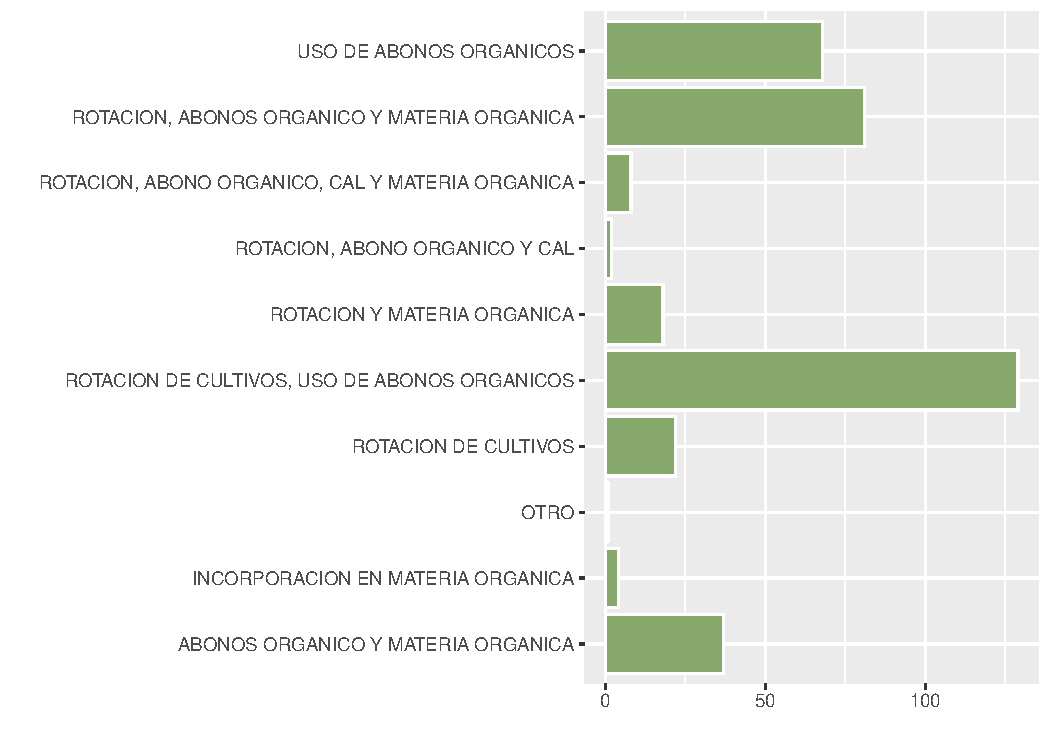
\includegraphics[width=\maxwidth]{figure/fig_treintaycuatro-1} 
\end{knitrout}
}
\end{graficas}

\begin{fotos}
{socializacion del proyecto}{32}
\end{fotos}


\begin{tablas}
{Realiza manejo de post cosecha}{

\begin{tabular}{lcl}
\toprule
\cellcolor[HTML]{87A96B}{\textcolor{black}{\textbf{Manejo}}} & \cellcolor[HTML]{87A96B}{\textcolor{black}{\textbf{Conteo}}} & \cellcolor[HTML]{87A96B}{\textcolor{black}{\textbf{Porcentaje}}}\\
\midrule
NO & 229 & 55.18\\
SI & 186 & 44.82\\
\bottomrule
\end{tabular}


}
\end{tablas}

\begin{graficas}
{Realiza manejo de post cosecha}{
\begin{knitrout}
\definecolor{shadecolor}{rgb}{0.969, 0.969, 0.969}\color{fgcolor}
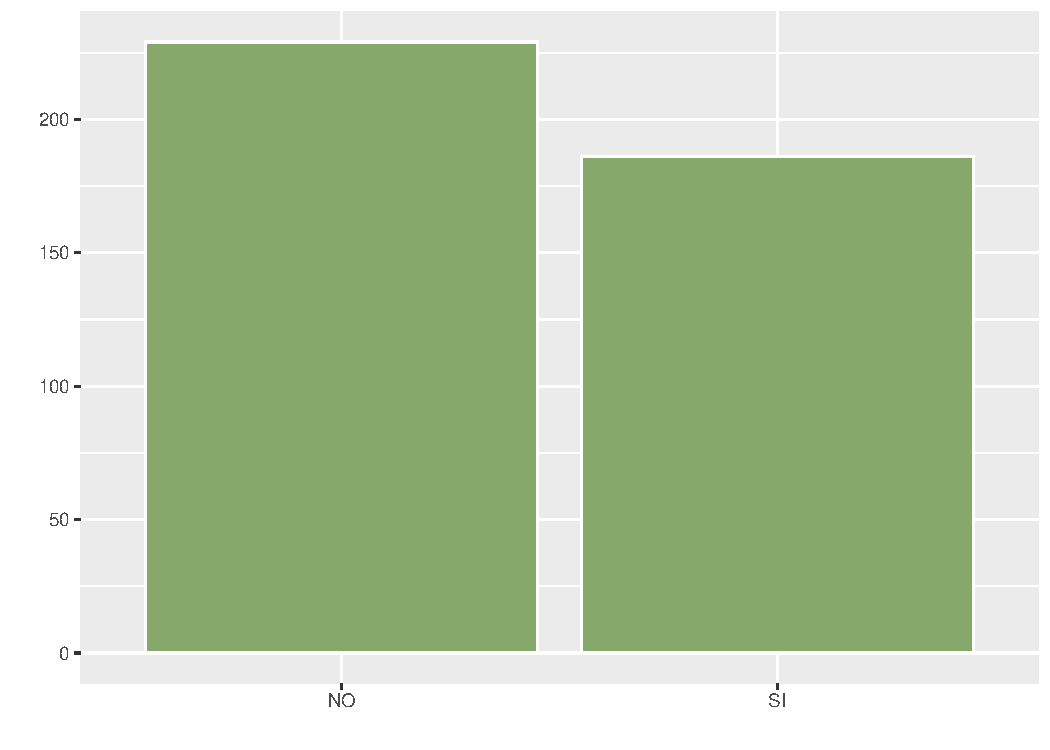
\includegraphics[width=\maxwidth]{figure/fig_treintaycinco-1} 
\end{knitrout}
}
\end{graficas}

\begin{fotos}
{socializacion del proyecto}{33}
\end{fotos}


\begin{tablas}
{Ha recibido alguna capacitacion}{

\begin{tabular}{lcl}
\toprule
\cellcolor[HTML]{87A96B}{\textcolor{black}{\textbf{Capacitacion}}} & \cellcolor[HTML]{87A96B}{\textcolor{black}{\textbf{Conteo}}} & \cellcolor[HTML]{87A96B}{\textcolor{black}{\textbf{Porcentaje}}}\\
\midrule
NO & 314 & 71.04\\
SI & 128 & 28.96\\
\bottomrule
\end{tabular}


}
\end{tablas}

\begin{graficas}
{Ha recibido alguna capacitacion}{
\begin{knitrout}
\definecolor{shadecolor}{rgb}{0.969, 0.969, 0.969}\color{fgcolor}
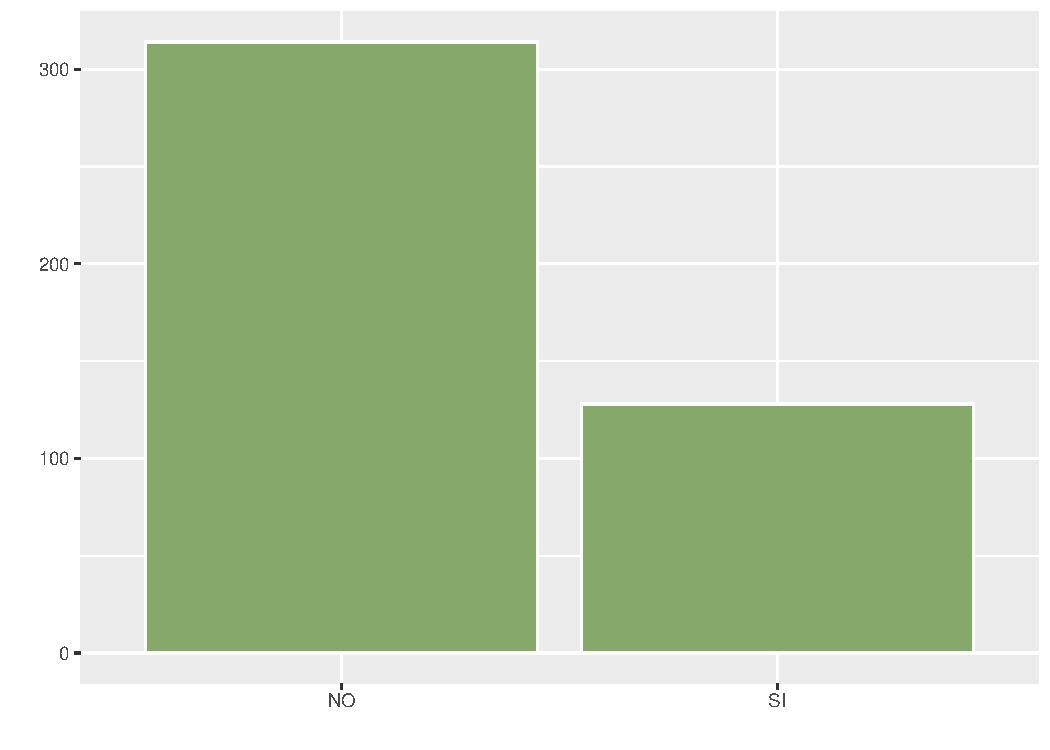
\includegraphics[width=\maxwidth]{figure/fig_treintayseis-1} 
\end{knitrout}
}
\end{graficas}

\begin{fotos}
{trabajo de campo}{34}
\end{fotos}

\begin{comment}

\begin{tablas}
{Temas de capacitacion}{

\begin{tabular}{lcl}
\toprule
\cellcolor[HTML]{87A96B}{\textcolor{black}{\textbf{Temas}}} & \cellcolor[HTML]{87A96B}{\textcolor{black}{\textbf{Conteo}}} & \cellcolor[HTML]{87A96B}{\textcolor{black}{\textbf{Porcentaje}}}\\
\midrule
CONTROL FITOSANITARIO & 2 & 1.48\\
CONTROL FITOSANITARIO, COSECHA & 1 & 0.74\\
FERTILIZACION Y ABONAMIENTO & 4 & 2.96\\
FERTILIZACION Y ABONAMIENTO, CONTROL FITOSANITARIO & 1 & 0.74\\
FERTILIZACION Y ABONAMIENTO, MEJORAMIENTO GENETICO & 1 & 0.74\\
\addlinespace
MEJORAMIENTO GENETICO & 2 & 1.48\\
OTRO & 13 & 9.63\\
PREPARACION DE TERRENO & 6 & 4.44\\
PREPARACION DE TERRENO, COSECHA & 1 & 0.74\\
PREPARACION DE TERRENO, MEJORAMIENTO GENETICO & 1 & 0.74\\
\addlinespace
PREPARACION DE TERRENO, SIEMBRA & 12 & 8.89\\
PREPARACION DE TERRENO, SIEMBRA, COSECHA & 17 & 12.59\\
PREPARACION DE TERRENO, SIEMBRA, COSECHA, MEJORAMIENTO GENETICO & 1 & 0.74\\
PREPARACION DE TERRENO, SIEMBRA, FERTILIZACION Y ABONAMIENTO & 3 & 2.22\\
PREPARACION DE TERRENO, SIEMBRA, FERTILIZACION Y ABONAMIENTO, CONTROL FITOSANITARIO & 5 & 3.70\\
\addlinespace
PREPARACION DE TERRENO, SIEMBRA, FERTILIZACION Y ABONAMIENTO, CONTROL FITOSANITARIO, COSECHA & 11 & 8.15\\
PREPARACION DE TERRENO, SIEMBRA, FERTILIZACION Y ABONAMIENTO, CONTROL FITOSANITARIO, MEJORAMIENTO GENETICO & 1 & 0.74\\
PREPARACION DE TERRENO, SIEMBRA, FERTILIZACION Y ABONAMIENTO, COSECHA & 11 & 8.15\\
PREPARACION DE TERRENO, SIEMBRA, FERTILIZACION Y ABONAMIENTO, COSECHA, MEJORAMIENTO GENETICO & 4 & 2.96\\
PREPARACION DE TERRENO, SIEMBRA, FERTILIZACION Y ABONAMIENTO, MEJORAMIENTO GENETICO & 3 & 2.22\\
\addlinespace
PREPARACION DE TERRENO, SIEMBRA, OTRO & 1 & 0.74\\
SIEMBRA & 7 & 5.19\\
SIEMBRA, CONTROL FITOSANITARIO & 1 & 0.74\\
SIEMBRA, COSECHA & 2 & 1.48\\
SIEMBRA, FERTILIZACION Y ABONAMIENTO & 1 & 0.74\\
\addlinespace
SIEMBRA, FERTILIZACION Y ABONAMIENTO, CONTROL FITOSANITARIO, COSECHA & 2 & 1.48\\
TERRENO Y FERTILIZACION & 2 & 1.48\\
TERRENO, FERTILIZACION, COSECHA & 4 & 2.96\\
TERRENO, FERTILIZACION, COSECHA, GENETICA & 1 & 0.74\\
TERRENO, FERTILIZACION, FITOSANITARIO, COSECHA & 1 & 0.74\\
\addlinespace
TERRENO, SIEMBRA, FERTILIZACION, FITOSANITARIO, COSECHA, GENETICA & 12 & 8.89\\
TERRENO, SIEMBRA, FITOSANITARIO & 1 & 0.74\\
\bottomrule
\end{tabular}


}
\end{tablas}

\begin{graficas}
{Temas de capacitacion}{
\begin{knitrout}
\definecolor{shadecolor}{rgb}{0.969, 0.969, 0.969}\color{fgcolor}
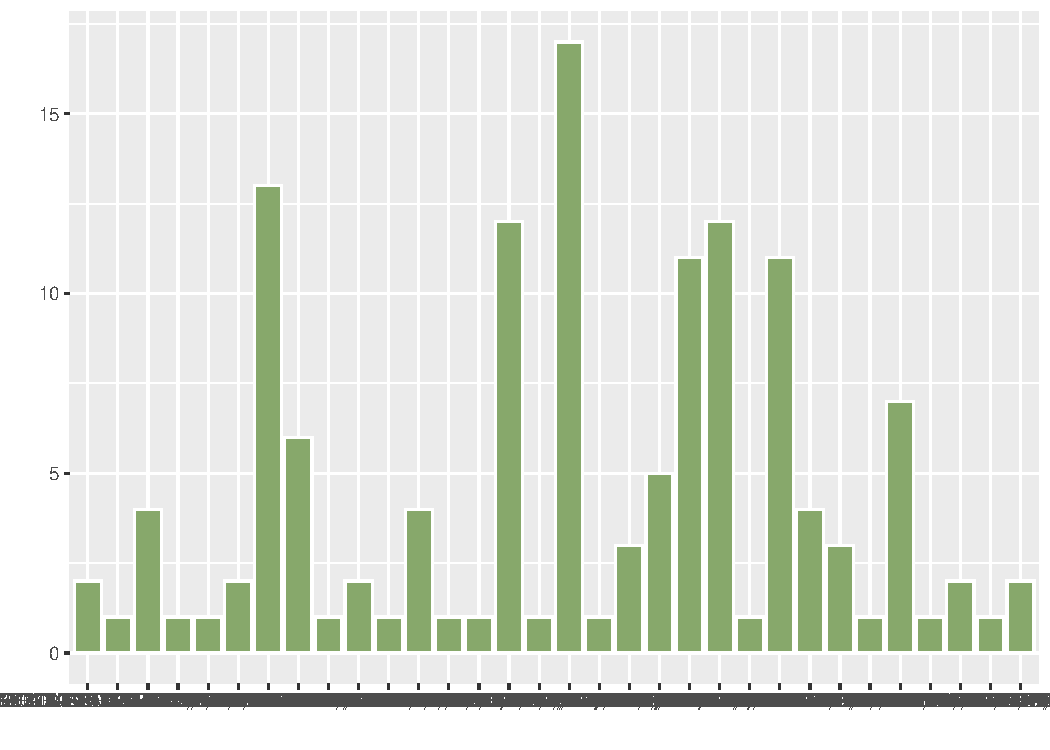
\includegraphics[width=\maxwidth]{figure/fig_treintaysiete-1} 
\end{knitrout}
}
\end{graficas}

\begin{fotos}
{trabajo de campo}{35}
\end{fotos}

\end{comment}

\begin{tablas}
{Donde realiza la comercializacion de su cosecha}{

\begin{tabular}{lcl}
\toprule
\cellcolor[HTML]{87A96B}{\textcolor{black}{\textbf{Lugar}}} & \cellcolor[HTML]{87A96B}{\textcolor{black}{\textbf{Conteo}}} & \cellcolor[HTML]{87A96B}{\textcolor{black}{\textbf{Porcentaje}}}\\
\midrule
EN MERCADOS LOCALES & 191 & 67.73\\
FERIAS AGROPECUARIAS & 16 & 5.67\\
OTRO & 6 & 2.13\\
VENTA EN LA PARCELA (CHACRA) & 40 & 14.18\\
VENTAS EN MERCADOS REGIONALES & 29 & 10.28\\
\bottomrule
\end{tabular}


}
\end{tablas}

\begin{graficas}
{Donde realiza la comercializacion de su cosecha}{
\begin{knitrout}
\definecolor{shadecolor}{rgb}{0.969, 0.969, 0.969}\color{fgcolor}
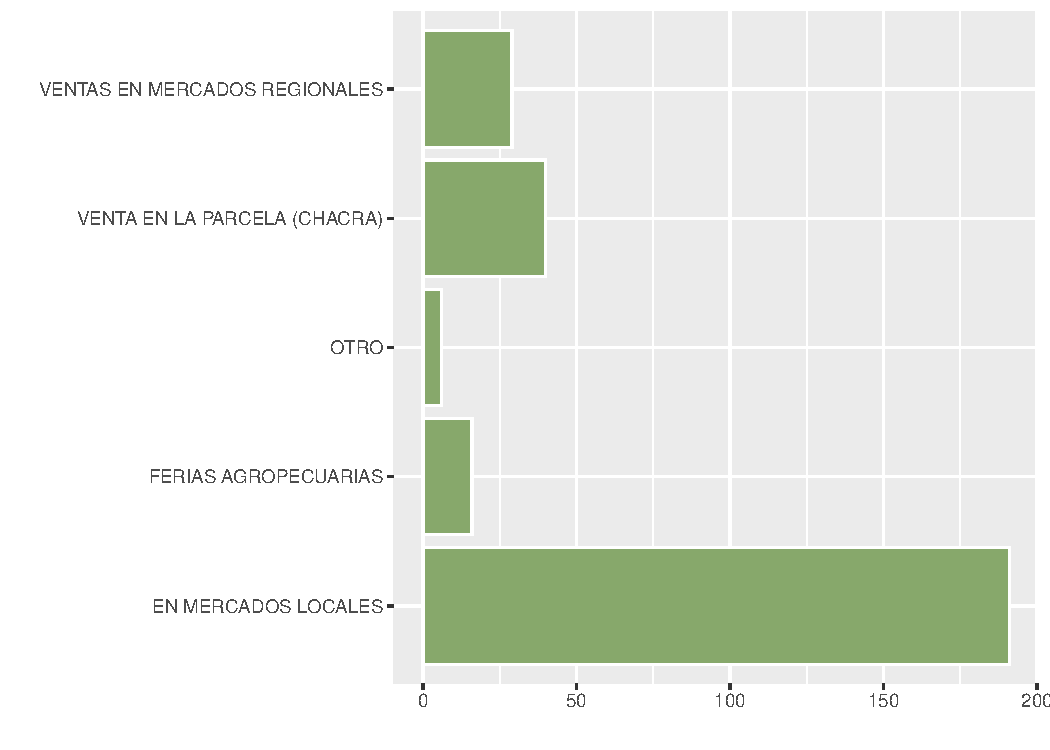
\includegraphics[width=\maxwidth]{figure/fig_treintayocho-1} 
\end{knitrout}
}
\end{graficas}

\begin{fotos}
{trabajo de campo}{36}
\end{fotos}


\begin{tablas}
{Pertenece a alguna organizacion o asociacion}{

\begin{tabular}{lcl}
\toprule
\cellcolor[HTML]{87A96B}{\textcolor{black}{\textbf{Pertenece}}} & \cellcolor[HTML]{87A96B}{\textcolor{black}{\textbf{Conteo}}} & \cellcolor[HTML]{87A96B}{\textcolor{black}{\textbf{Porcentaje}}}\\
\midrule
NO & 273 & 68.77\\
SI & 124 & 31.23\\
\bottomrule
\end{tabular}


}
\end{tablas}

\begin{graficas}
{Pertenece a alguna organizacion o asociacion}{
\begin{knitrout}
\definecolor{shadecolor}{rgb}{0.969, 0.969, 0.969}\color{fgcolor}
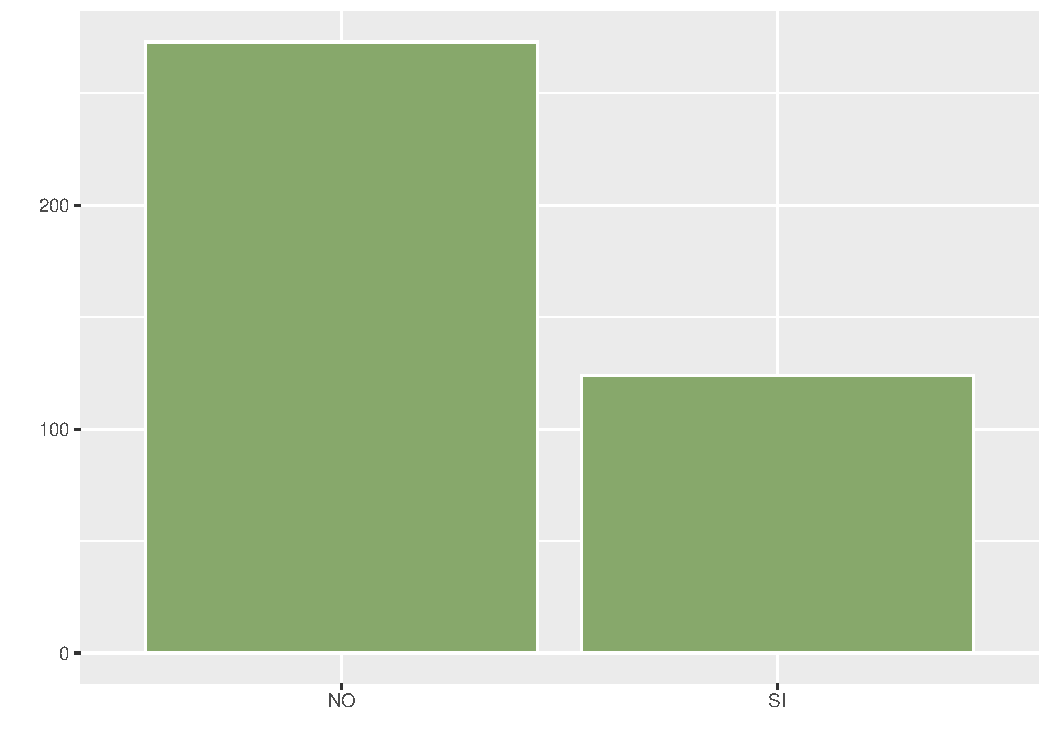
\includegraphics[width=\maxwidth]{figure/fig_treintaynueve-1} 
\end{knitrout}
}
\end{graficas}

\begin{fotos}
{trabajo de campo}{37}
\end{fotos}

\begin{comment}

\begin{tablas}
{Meses en los que realiza la cosecha}{

\begin{tabular}{lcl}
\toprule
\cellcolor[HTML]{87A96B}{\textcolor{black}{\textbf{Meses}}} & \cellcolor[HTML]{87A96B}{\textcolor{black}{\textbf{Conteo}}} & \cellcolor[HTML]{87A96B}{\textcolor{black}{\textbf{Porcentaje}}}\\
\midrule
ABRIL & 15 & 3.53\\
ABRIL, AGOSTO, DICIEMBRE & 2 & 0.47\\
ABRIL, DICIEMBRE & 1 & 0.24\\
ABRIL, MAYO & 18 & 4.24\\
ABRIL, MAYO, JUNIO & 12 & 2.82\\
\addlinespace
ABRIL, MAYO, JUNIO, JULIO & 1 & 0.24\\
ABRIL, MAYO, JUNIO, JULIO, AGOSTO, SETIEMBRE & 1 & 0.24\\
AGOSTO & 2 & 0.47\\
ENERO, ABRIL, MAYO, SETIEMBRE & 1 & 0.24\\
ENERO, AGOSTO, DICIEMBRE & 1 & 0.24\\
\addlinespace
ENERO, DICIEMBRE & 1 & 0.24\\
ENERO, FEBRERO, MARZO & 1 & 0.24\\
ENERO, FEBRERO, MARZO, ABRIL & 1 & 0.24\\
ENERO, FEBRERO, MARZO, ABRIL, MAYO & 1 & 0.24\\
ENERO, FEBRERO, MARZO, ABRIL, MAYO, JUNIO & 5 & 1.18\\
\addlinespace
ENERO, FEBRERO, MARZO, ABRIL, MAYO, JUNIO, JULIO & 10 & 2.35\\
ENERO, FEBRERO, MARZO, ABRIL, MAYO, JUNIO, JULIO, AGOSTO & 2 & 0.47\\
ENERO, FEBRERO, MARZO, ABRIL, MAYO, JUNIO, JULIO, AGOSTO, SETIEMBRE, OCTUBRE, DICIEMBRE & 35 & 8.24\\
ENERO, FEBRERO, MARZO, MAYO, AGOSTO, DICIEMBRE & 1 & 0.24\\
ENERO, FEBRERO, MARZO, MAYO, JUNIO & 1 & 0.24\\
\addlinespace
ENERO, FEBRERO, MARZO, MAYO, JUNIO, JULIO & 3 & 0.71\\
ENERO, FEBRERO, MAYO & 1 & 0.24\\
ENERO, FEBRERO, MAYO, JUNIO, JULIO & 2 & 0.47\\
ENERO, FEBRERO, MAYO, JUNIO, JULIO, DICIEMBRE & 1 & 0.24\\
ENERO, MAYO, DICIEMBRE & 2 & 0.47\\
\addlinespace
FEBRERO & 5 & 1.18\\
FEBRERO, MARZO & 4 & 0.94\\
FEBRERO, MARZO, ABRIL & 1 & 0.24\\
FEBRERO, MARZO, MAYO, JUNIO & 1 & 0.24\\
FEBRERO, MAYO & 2 & 0.47\\
\addlinespace
JULIO & 3 & 0.71\\
JULIO, AGOSTO & 1 & 0.24\\
JUNIO & 57 & 13.41\\
JUNIO, DICIEMBRE & 2 & 0.47\\
JUNIO, JULIO & 19 & 4.47\\
\addlinespace
JUNIO, JULIO, AGOSTO & 3 & 0.71\\
MARZO & 1 & 0.24\\
MARZO, ABRIL & 4 & 0.94\\
MARZO, ABRIL, MAYO & 1 & 0.24\\
MARZO, ABRIL, MAYO, JUNIO & 2 & 0.47\\
\addlinespace
MARZO, ABRIL, MAYO, JUNIO, JULIO & 1 & 0.24\\
MARZO, JULIO, OCTUBRE & 1 & 0.24\\
MARZO, JUNIO & 1 & 0.24\\
MARZO, JUNIO, JULIO & 1 & 0.24\\
MARZO, MAYO, JULIO, SETIEMBRE & 1 & 0.24\\
\addlinespace
MARZO, MAYO, JUNIO, JULIO, DICIEMBRE & 1 & 0.24\\
MARZO, MAYO, OCTUBRE & 1 & 0.24\\
MAYO & 93 & 21.88\\
MAYO, JULIO & 2 & 0.47\\
MAYO, JUNIO & 81 & 19.06\\
\addlinespace
MAYO, JUNIO, AGOSTO, OCTUBRE & 1 & 0.24\\
MAYO, JUNIO, DICIEMBRE & 1 & 0.24\\
MAYO, JUNIO, JULIO & 9 & 2.12\\
MAYO, JUNIO, JULIO, AGOSTO & 3 & 0.71\\
OCTUBRE & 1 & 0.24\\
\bottomrule
\end{tabular}


}
\end{tablas}

\begin{graficas}
{Meses en los que realiza la cosecha}{
\begin{knitrout}
\definecolor{shadecolor}{rgb}{0.969, 0.969, 0.969}\color{fgcolor}
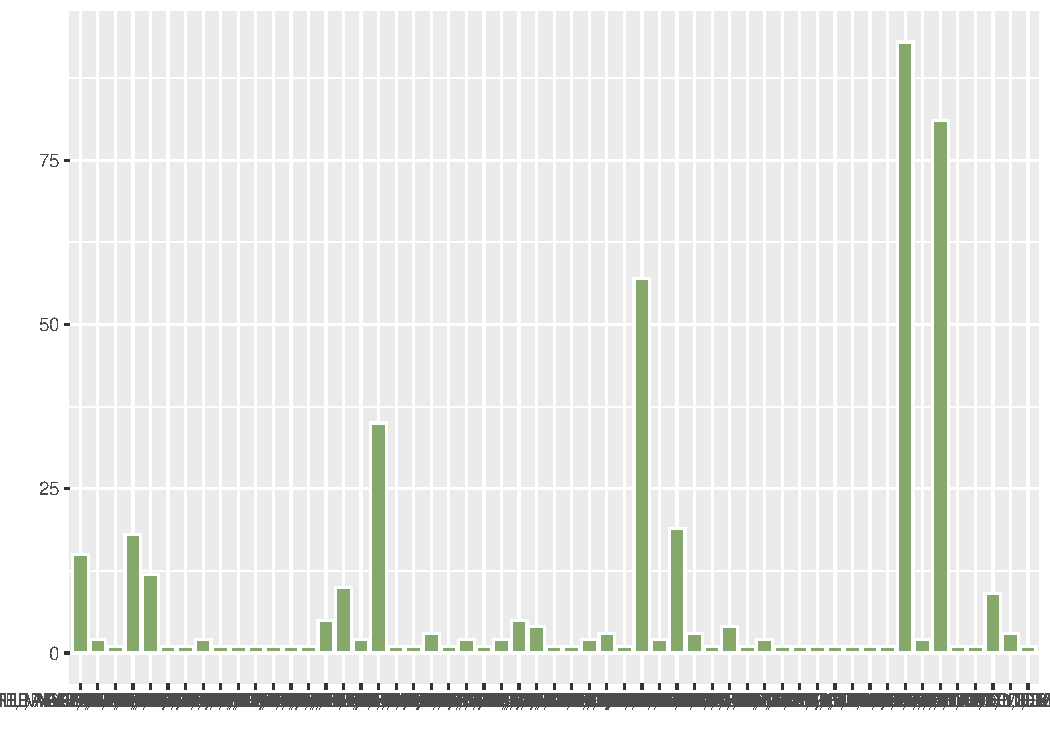
\includegraphics[width=\maxwidth]{figure/fig_cuarenta-1} 
\end{knitrout}
}
\end{graficas}

\begin{fotos}
{trabajo de campo}{38}
\end{fotos}

\end{comment}

\begin{tablas}
{Insumos que usa para la produccion y cosecha}{

\begin{tabular}{lcl}
\toprule
\cellcolor[HTML]{87A96B}{\textcolor{black}{\textbf{Insumo}}} & \cellcolor[HTML]{87A96B}{\textcolor{black}{\textbf{Conteo}}} & \cellcolor[HTML]{87A96B}{\textcolor{black}{\textbf{Porcentaje}}}\\
\midrule
ANIMALES Y HERRAMIENTAS & 105 & 26.05\\
ANIMALES Y MAQUINARIA AGRICOLA & 3 & 0.74\\
HERRAMIENTAS MANUALES & 59 & 14.64\\
HERRAMIENTAS Y MAQUINARIA AGRICOLA & 113 & 28.04\\
HERRAMIENTAS, ANIMALES Y MAQUINARIA AGRICOLA & 96 & 23.82\\
\addlinespace
IMPLEMENTOS TIRADO POR ANIMALES & 3 & 0.74\\
MAQUINARIA AGRICOLA & 24 & 5.96\\
\bottomrule
\end{tabular}


}
\end{tablas}

\begin{graficas}
{Insumos que usa para la produccion y cosecha}{
\begin{knitrout}
\definecolor{shadecolor}{rgb}{0.969, 0.969, 0.969}\color{fgcolor}
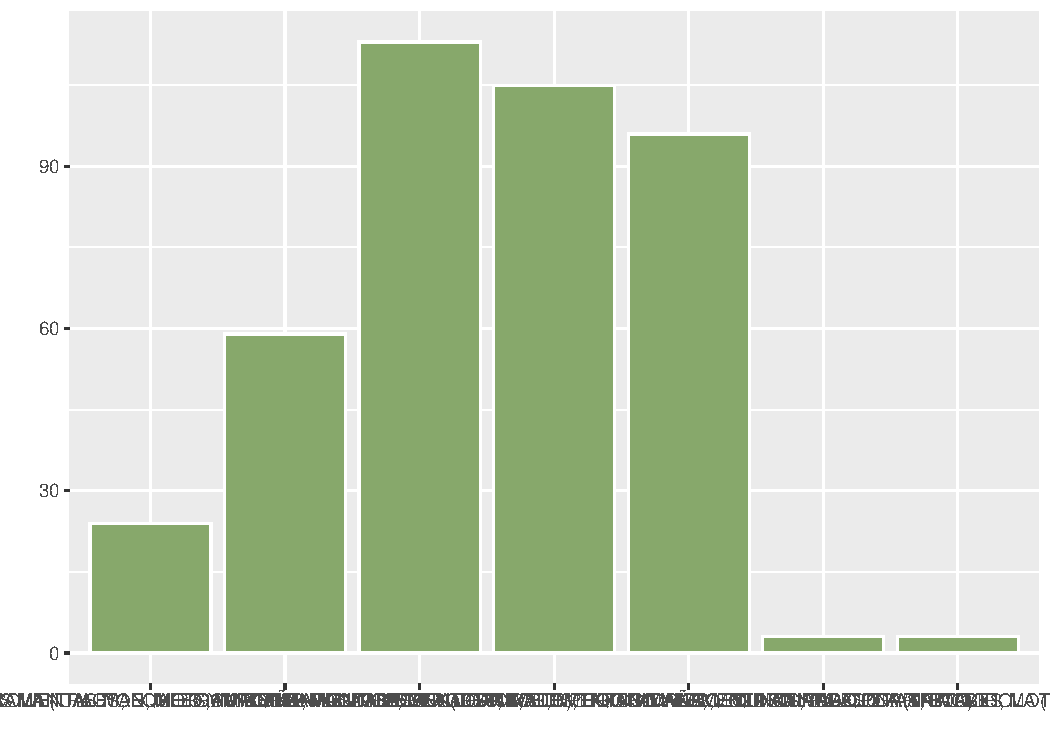
\includegraphics[width=\maxwidth]{figure/fig_cuarentayuno-1} 
\end{knitrout}
}
\end{graficas}

\begin{fotos}
{trabajo de campo}{39}
\end{fotos}

%para hacer commit desde la terminal:
%git add .
%git commit -m "Actualizacion de archivos (esto se puede modificar) .Rnw"
%para hacer push
%git push origin main



\end{document}
